% Options for packages loaded elsewhere
\PassOptionsToPackage{unicode}{hyperref}
\PassOptionsToPackage{hyphens}{url}
%
\documentclass[
]{book}
\usepackage{amsmath,amssymb}
\usepackage{iftex}
\ifPDFTeX
  \usepackage[T1]{fontenc}
  \usepackage[utf8]{inputenc}
  \usepackage{textcomp} % provide euro and other symbols
\else % if luatex or xetex
  \usepackage{unicode-math} % this also loads fontspec
  \defaultfontfeatures{Scale=MatchLowercase}
  \defaultfontfeatures[\rmfamily]{Ligatures=TeX,Scale=1}
\fi
\usepackage{lmodern}
\ifPDFTeX\else
  % xetex/luatex font selection
\fi
% Use upquote if available, for straight quotes in verbatim environments
\IfFileExists{upquote.sty}{\usepackage{upquote}}{}
\IfFileExists{microtype.sty}{% use microtype if available
  \usepackage[]{microtype}
  \UseMicrotypeSet[protrusion]{basicmath} % disable protrusion for tt fonts
}{}
\makeatletter
\@ifundefined{KOMAClassName}{% if non-KOMA class
  \IfFileExists{parskip.sty}{%
    \usepackage{parskip}
  }{% else
    \setlength{\parindent}{0pt}
    \setlength{\parskip}{6pt plus 2pt minus 1pt}}
}{% if KOMA class
  \KOMAoptions{parskip=half}}
\makeatother
\usepackage{xcolor}
\usepackage{color}
\usepackage{fancyvrb}
\newcommand{\VerbBar}{|}
\newcommand{\VERB}{\Verb[commandchars=\\\{\}]}
\DefineVerbatimEnvironment{Highlighting}{Verbatim}{commandchars=\\\{\}}
% Add ',fontsize=\small' for more characters per line
\usepackage{framed}
\definecolor{shadecolor}{RGB}{248,248,248}
\newenvironment{Shaded}{\begin{snugshade}}{\end{snugshade}}
\newcommand{\AlertTok}[1]{\textcolor[rgb]{0.94,0.16,0.16}{#1}}
\newcommand{\AnnotationTok}[1]{\textcolor[rgb]{0.56,0.35,0.01}{\textbf{\textit{#1}}}}
\newcommand{\AttributeTok}[1]{\textcolor[rgb]{0.13,0.29,0.53}{#1}}
\newcommand{\BaseNTok}[1]{\textcolor[rgb]{0.00,0.00,0.81}{#1}}
\newcommand{\BuiltInTok}[1]{#1}
\newcommand{\CharTok}[1]{\textcolor[rgb]{0.31,0.60,0.02}{#1}}
\newcommand{\CommentTok}[1]{\textcolor[rgb]{0.56,0.35,0.01}{\textit{#1}}}
\newcommand{\CommentVarTok}[1]{\textcolor[rgb]{0.56,0.35,0.01}{\textbf{\textit{#1}}}}
\newcommand{\ConstantTok}[1]{\textcolor[rgb]{0.56,0.35,0.01}{#1}}
\newcommand{\ControlFlowTok}[1]{\textcolor[rgb]{0.13,0.29,0.53}{\textbf{#1}}}
\newcommand{\DataTypeTok}[1]{\textcolor[rgb]{0.13,0.29,0.53}{#1}}
\newcommand{\DecValTok}[1]{\textcolor[rgb]{0.00,0.00,0.81}{#1}}
\newcommand{\DocumentationTok}[1]{\textcolor[rgb]{0.56,0.35,0.01}{\textbf{\textit{#1}}}}
\newcommand{\ErrorTok}[1]{\textcolor[rgb]{0.64,0.00,0.00}{\textbf{#1}}}
\newcommand{\ExtensionTok}[1]{#1}
\newcommand{\FloatTok}[1]{\textcolor[rgb]{0.00,0.00,0.81}{#1}}
\newcommand{\FunctionTok}[1]{\textcolor[rgb]{0.13,0.29,0.53}{\textbf{#1}}}
\newcommand{\ImportTok}[1]{#1}
\newcommand{\InformationTok}[1]{\textcolor[rgb]{0.56,0.35,0.01}{\textbf{\textit{#1}}}}
\newcommand{\KeywordTok}[1]{\textcolor[rgb]{0.13,0.29,0.53}{\textbf{#1}}}
\newcommand{\NormalTok}[1]{#1}
\newcommand{\OperatorTok}[1]{\textcolor[rgb]{0.81,0.36,0.00}{\textbf{#1}}}
\newcommand{\OtherTok}[1]{\textcolor[rgb]{0.56,0.35,0.01}{#1}}
\newcommand{\PreprocessorTok}[1]{\textcolor[rgb]{0.56,0.35,0.01}{\textit{#1}}}
\newcommand{\RegionMarkerTok}[1]{#1}
\newcommand{\SpecialCharTok}[1]{\textcolor[rgb]{0.81,0.36,0.00}{\textbf{#1}}}
\newcommand{\SpecialStringTok}[1]{\textcolor[rgb]{0.31,0.60,0.02}{#1}}
\newcommand{\StringTok}[1]{\textcolor[rgb]{0.31,0.60,0.02}{#1}}
\newcommand{\VariableTok}[1]{\textcolor[rgb]{0.00,0.00,0.00}{#1}}
\newcommand{\VerbatimStringTok}[1]{\textcolor[rgb]{0.31,0.60,0.02}{#1}}
\newcommand{\WarningTok}[1]{\textcolor[rgb]{0.56,0.35,0.01}{\textbf{\textit{#1}}}}
\usepackage{longtable,booktabs,array}
\usepackage{calc} % for calculating minipage widths
% Correct order of tables after \paragraph or \subparagraph
\usepackage{etoolbox}
\makeatletter
\patchcmd\longtable{\par}{\if@noskipsec\mbox{}\fi\par}{}{}
\makeatother
% Allow footnotes in longtable head/foot
\IfFileExists{footnotehyper.sty}{\usepackage{footnotehyper}}{\usepackage{footnote}}
\makesavenoteenv{longtable}
\usepackage{graphicx}
\makeatletter
\def\maxwidth{\ifdim\Gin@nat@width>\linewidth\linewidth\else\Gin@nat@width\fi}
\def\maxheight{\ifdim\Gin@nat@height>\textheight\textheight\else\Gin@nat@height\fi}
\makeatother
% Scale images if necessary, so that they will not overflow the page
% margins by default, and it is still possible to overwrite the defaults
% using explicit options in \includegraphics[width, height, ...]{}
\setkeys{Gin}{width=\maxwidth,height=\maxheight,keepaspectratio}
% Set default figure placement to htbp
\makeatletter
\def\fps@figure{htbp}
\makeatother
\setlength{\emergencystretch}{3em} % prevent overfull lines
\providecommand{\tightlist}{%
  \setlength{\itemsep}{0pt}\setlength{\parskip}{0pt}}
\setcounter{secnumdepth}{5}
\usepackage{booktabs}
\usepackage{amsthm}
\makeatletter
\def\thm@space@setup{%
  \thm@preskip=8pt plus 2pt minus 4pt
  \thm@postskip=\thm@preskip
}
\makeatother
\ifLuaTeX
  \usepackage{selnolig}  % disable illegal ligatures
\fi
\usepackage[]{natbib}
\bibliographystyle{plainnat}
\IfFileExists{bookmark.sty}{\usepackage{bookmark}}{\usepackage{hyperref}}
\IfFileExists{xurl.sty}{\usepackage{xurl}}{} % add URL line breaks if available
\urlstyle{same}
\hypersetup{
  pdftitle={PSC 253 Minimal Manual},
  pdfauthor={Matthew B. Platt},
  hidelinks,
  pdfcreator={LaTeX via pandoc}}

\title{PSC 253 Minimal Manual}
\author{Matthew B. Platt}
\date{2024-10-12}

\begin{document}
\maketitle

{
\setcounter{tocdepth}{1}
\tableofcontents
}
\hypertarget{preface}{%
\chapter*{Preface}\label{preface}}
\addcontentsline{toc}{chapter}{Preface}

This book is a supplement to the book, \href{http://qss.princeton.press/}{Quantitative Social Science: An Introduction}, by Kosuke Imai. It also relies heavily on the work of \href{https://jrnold.github.io/qss-tidy/}{Jeffrey Arnold}, who translated the Imai code into tidyverse code.

This manual is also a supplement to the book \href{https://us.sagepub.com/en-us/nam/an-r-companion-to-political-analysis/book244716}{An R Companion to Political Analysis} by Philip Pollock III and Barry Edwards.

I aspire for this text to act as a minimal manual for the course PSC 253 Scope and Methods in Political Science taught at Morehouse College. It is intended to cover all of the main analytical tasks that the course requires.

\hypertarget{basic}{%
\chapter{R Basics}\label{basic}}

At its most basic functionality, R is a calculator.

\hypertarget{calculate}{%
\section{Use R as a Calculator}\label{calculate}}

\hypertarget{problem}{%
\subsection{Problem}\label{problem}}

You want to add, subtract, multiply, divide, use exponents, and take square roots

\hypertarget{solution}{%
\subsection{Solution}\label{solution}}

Use \texttt{+} for addition, \texttt{-} for subtraction, \texttt{*} for multiplication and \texttt{/} for division.

\begin{Shaded}
\begin{Highlighting}[]
\CommentTok{\# addition}
\DecValTok{43} \SpecialCharTok{+} \DecValTok{5}
\end{Highlighting}
\end{Shaded}

\begin{verbatim}
## [1] 48
\end{verbatim}

\begin{Shaded}
\begin{Highlighting}[]
\CommentTok{\# subtraction}
\DecValTok{43} \SpecialCharTok{{-}} \DecValTok{5}
\end{Highlighting}
\end{Shaded}

\begin{verbatim}
## [1] 38
\end{verbatim}

\begin{Shaded}
\begin{Highlighting}[]
\CommentTok{\# multiplication}
\DecValTok{43} \SpecialCharTok{*} \DecValTok{5}
\end{Highlighting}
\end{Shaded}

\begin{verbatim}
## [1] 215
\end{verbatim}

\begin{Shaded}
\begin{Highlighting}[]
\CommentTok{\# division}
\DecValTok{43}\SpecialCharTok{/}\DecValTok{5}
\end{Highlighting}
\end{Shaded}

\begin{verbatim}
## [1] 8.6
\end{verbatim}

For exponents, we raise \texttt{X} to the power of \texttt{y} by using \texttt{\^{}}. That is \texttt{X\^{}y}.

\begin{Shaded}
\begin{Highlighting}[]
\CommentTok{\# raise 43 to the power of 5}
\DecValTok{43} \SpecialCharTok{\^{}} \DecValTok{5}
\end{Highlighting}
\end{Shaded}

\begin{verbatim}
## [1] 147008443
\end{verbatim}

Take the square root of some number \texttt{x} by using the function \texttt{sqrt()}. That is \texttt{sqrt(x)}.

\begin{Shaded}
\begin{Highlighting}[]
\CommentTok{\# take the square root of 43}
\FunctionTok{sqrt}\NormalTok{(}\DecValTok{43}\NormalTok{)}
\end{Highlighting}
\end{Shaded}

\begin{verbatim}
## [1] 6.557439
\end{verbatim}

\hypertarget{troubleshooting}{%
\subsection{Troubleshooting}\label{troubleshooting}}

\begin{itemize}
\tightlist
\item
  Keep in mind that R follows the order of operations, 2 + 2 * 2 is equal to 6 and not 8.
\end{itemize}

\begin{Shaded}
\begin{Highlighting}[]
\CommentTok{\# correct}
\DecValTok{2} \SpecialCharTok{+} \DecValTok{2} \SpecialCharTok{*} \DecValTok{2}
\end{Highlighting}
\end{Shaded}

\begin{verbatim}
## [1] 6
\end{verbatim}

\begin{Shaded}
\begin{Highlighting}[]
\CommentTok{\# incorrect}
\NormalTok{(}\DecValTok{2} \SpecialCharTok{+} \DecValTok{2}\NormalTok{) }\SpecialCharTok{*} \DecValTok{2}
\end{Highlighting}
\end{Shaded}

\begin{verbatim}
## [1] 8
\end{verbatim}

\hypertarget{object}{%
\section{Creating an Object}\label{object}}

\hypertarget{problem-1}{%
\subsection{Problem}\label{problem-1}}

You want to create an object to hold a number

\hypertarget{solution-1}{%
\subsection{Solution}\label{solution-1}}

To create an object:

\begin{enumerate}
\def\labelenumi{\arabic{enumi}.}
\tightlist
\item
  type in a name for the object, like \texttt{newobject} then
\item
  use the assignment operator \texttt{\textless{}-},
\item
  input a number, mathematical expression, dataset, or text on the right side of \texttt{\textless{}-} that you want assigned to the \texttt{newobject}
\end{enumerate}

\begin{Shaded}
\begin{Highlighting}[]
\CommentTok{\# assigning the number 4 to a new object named "myobject"}
\NormalTok{myobject }\OtherTok{\textless{}{-}} \DecValTok{4}

\CommentTok{\# assigning the text "hallelujah hollaback" to a new object named "second\_object"}
\NormalTok{second\_object }\OtherTok{\textless{}{-}} \StringTok{"hallelujah hollaback"}
\end{Highlighting}
\end{Shaded}

Type the name of an object in order to see what it contains.

\begin{Shaded}
\begin{Highlighting}[]
\NormalTok{myobject}
\end{Highlighting}
\end{Shaded}

\begin{verbatim}
## [1] 4
\end{verbatim}

\begin{Shaded}
\begin{Highlighting}[]
\NormalTok{second\_object}
\end{Highlighting}
\end{Shaded}

\begin{verbatim}
## [1] "hallelujah hollaback"
\end{verbatim}

\hypertarget{troubleshooting-1}{%
\subsection{Troubleshooting}\label{troubleshooting-1}}

\begin{itemize}
\tightlist
\item
  There cannot be any spaces in the name of an object. Instead you could use dots, dashes, underscores, or capitalization to distinguish between words: \texttt{small.data}, \texttt{big-data}, \texttt{bigger\_data}, \texttt{mediumData}.
\item
  Text needs to be in quotation marks in order to be assigned to an object.
\item
  Object names are case sensitive \texttt{Myobject} is not the same as \texttt{myobject}
\end{itemize}

\hypertarget{vector}{%
\section{Creating a Vector}\label{vector}}

A vector is a list of numbers or characters. We will create vectors for a variety of reasons in this course.

\hypertarget{problem-2}{%
\subsection{Problem}\label{problem-2}}

You want to create a vector.

\hypertarget{solution-2}{%
\subsection{Solution}\label{solution-2}}

Use the function \texttt{c()} to create a list by separating the entries with a comma.

\begin{Shaded}
\begin{Highlighting}[]
\CommentTok{\# create a vector called \textquotesingle{}prime\textquotesingle{}}
\NormalTok{prime }\OtherTok{\textless{}{-}} \FunctionTok{c}\NormalTok{(}\DecValTok{1}\NormalTok{, }\DecValTok{3}\NormalTok{, }\DecValTok{5}\NormalTok{, }\DecValTok{7}\NormalTok{)}

\NormalTok{prime}
\end{Highlighting}
\end{Shaded}

\begin{verbatim}
## [1] 1 3 5 7
\end{verbatim}

\begin{Shaded}
\begin{Highlighting}[]
\CommentTok{\# create a vector called "first\_name"}
\NormalTok{first\_name }\OtherTok{\textless{}{-}} \FunctionTok{c}\NormalTok{(}\StringTok{"Matthew"}\NormalTok{, }\StringTok{"Mosi"}\NormalTok{, }\StringTok{"Manu"}\NormalTok{, }\StringTok{"Ekundayo"}\NormalTok{, }\StringTok{"Kwasi"}\NormalTok{)}

\NormalTok{first\_name}
\end{Highlighting}
\end{Shaded}

\begin{verbatim}
## [1] "Matthew"  "Mosi"     "Manu"     "Ekundayo" "Kwasi"
\end{verbatim}

\hypertarget{troubleshooting-2}{%
\subsection{Troubleshooting}\label{troubleshooting-2}}

\begin{itemize}
\tightlist
\item
  As the name of a function, \texttt{c()} is case sensitive. Use the lowercase \texttt{c}.
\item
  Make sure that all elements are separated by a comma.
\item
  Vectors are typically assigned to some object.
\end{itemize}

\hypertarget{indexing}{%
\section{Indexing}\label{indexing}}

We can use indexing to pull out specific sets of observations from a vector or dataset.

\hypertarget{problem-3}{%
\subsection{Problem}\label{problem-3}}

You want to select a specific one observation based on its position within a vector or matrix.

\hypertarget{solution-3}{%
\subsection{Solution}\label{solution-3}}

We index by using the brackets \texttt{{[}x,\ y{]}} after an object where x is the row and y is the column.

\begin{Shaded}
\begin{Highlighting}[]
\CommentTok{\# we have a vector}
\NormalTok{prime }\OtherTok{\textless{}{-}} \FunctionTok{c}\NormalTok{(}\DecValTok{1}\NormalTok{, }\DecValTok{3}\NormalTok{, }\DecValTok{5}\NormalTok{, }\DecValTok{7}\NormalTok{)}

\CommentTok{\# we want the number 3, which is the second observation in the vector}
\NormalTok{prime[}\DecValTok{2}\NormalTok{]}
\end{Highlighting}
\end{Shaded}

\begin{verbatim}
## [1] 3
\end{verbatim}

\begin{Shaded}
\begin{Highlighting}[]
\CommentTok{\# we have a matrix}
\NormalTok{yup }\OtherTok{\textless{}{-}} \FunctionTok{matrix}\NormalTok{(}\FunctionTok{c}\NormalTok{(prime,}\DecValTok{2}\NormalTok{, }\DecValTok{6}\NormalTok{, }\DecValTok{10}\NormalTok{, }\DecValTok{14}\NormalTok{), }\AttributeTok{nrow =} \DecValTok{2}\NormalTok{, }\AttributeTok{ncol =} \DecValTok{4}\NormalTok{, }\AttributeTok{byrow =}\NormalTok{ T)}
\NormalTok{yup}
\end{Highlighting}
\end{Shaded}

\begin{verbatim}
##      [,1] [,2] [,3] [,4]
## [1,]    1    3    5    7
## [2,]    2    6   10   14
\end{verbatim}

\begin{Shaded}
\begin{Highlighting}[]
\CommentTok{\# We want the observation in the first row and fourth column}
\NormalTok{yup[}\DecValTok{1}\NormalTok{, }\DecValTok{4}\NormalTok{]}
\end{Highlighting}
\end{Shaded}

\begin{verbatim}
## [1] 7
\end{verbatim}

\hypertarget{problem-4}{%
\subsection{Problem}\label{problem-4}}

You want to select an entire row or column.

\hypertarget{solution-4}{%
\subsection{Solution}\label{solution-4}}

You can select an entire row by leaving the column index position blank \texttt{yup{[}2,\ {]}}. You can select an entire column by leaving the row index position blank \texttt{yup{[}\ ,\ 2{]}}.

\begin{Shaded}
\begin{Highlighting}[]
\CommentTok{\# We have our matrix}
\NormalTok{yup}
\end{Highlighting}
\end{Shaded}

\begin{verbatim}
##      [,1] [,2] [,3] [,4]
## [1,]    1    3    5    7
## [2,]    2    6   10   14
\end{verbatim}

\begin{Shaded}
\begin{Highlighting}[]
\CommentTok{\# We want the second row}
\NormalTok{yup[}\DecValTok{1}\NormalTok{, ]}
\end{Highlighting}
\end{Shaded}

\begin{verbatim}
## [1] 1 3 5 7
\end{verbatim}

\begin{Shaded}
\begin{Highlighting}[]
\CommentTok{\# We want the third column}
\NormalTok{yup[ , }\DecValTok{3}\NormalTok{]}
\end{Highlighting}
\end{Shaded}

\begin{verbatim}
## [1]  5 10
\end{verbatim}

\hypertarget{project}{%
\section{Creating a Project}\label{project}}

Creating a project creates a folder on your computer that Rstudio and R will treat as the default directory for your code. That is, whenever you tell R to look for something on your computer, it will begin by looking in the project folder.

\hypertarget{problem-5}{%
\subsection{Problem}\label{problem-5}}

You want to create a new project.

\hypertarget{solution-5}{%
\subsection{Solution}\label{solution-5}}

There are multiple ways to create a new project. You can go to the menu bar and select ``File'', then ``New Project'':

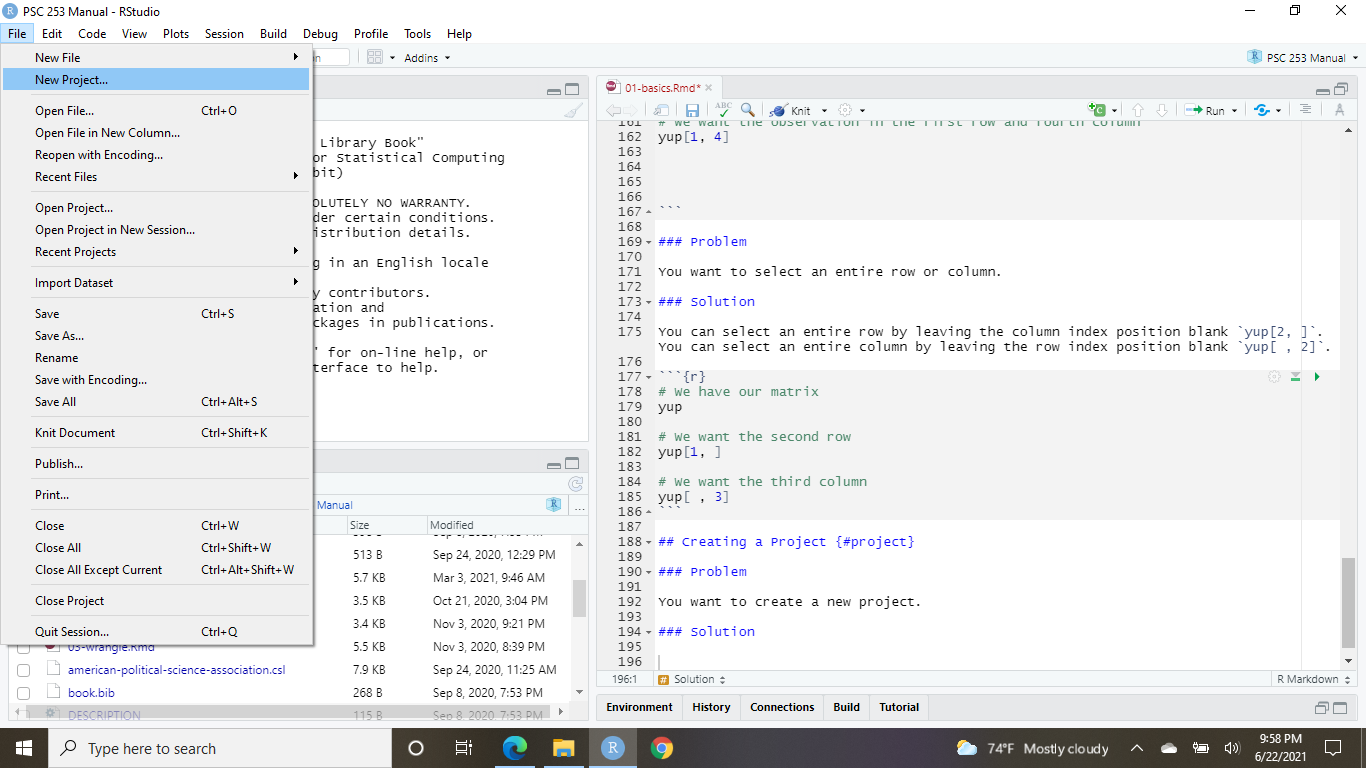
\includegraphics{images/projectfile.png}

You can click the ``create project'' icon on the toolbar:

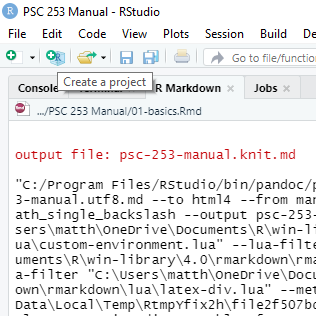
\includegraphics{images/projectbar.png}

Or you can select ``New Project'' from the project menu at the top left of Rstudio:

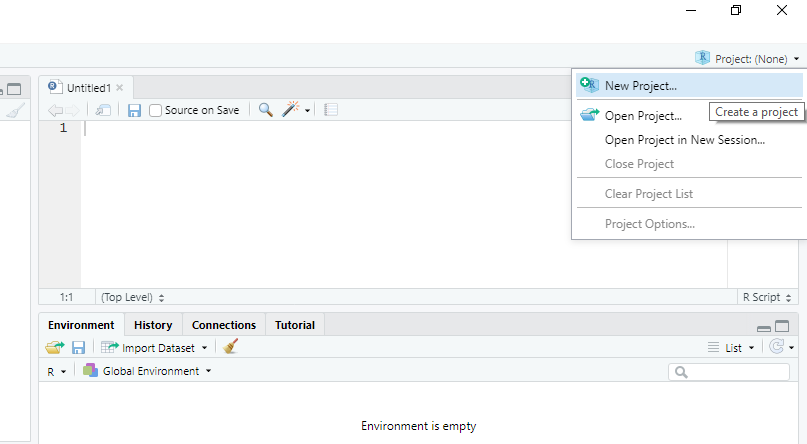
\includegraphics{images/projectmenu.png}

When you select ``New Project'', the below dialogue box appears. Select ``New Directory'':

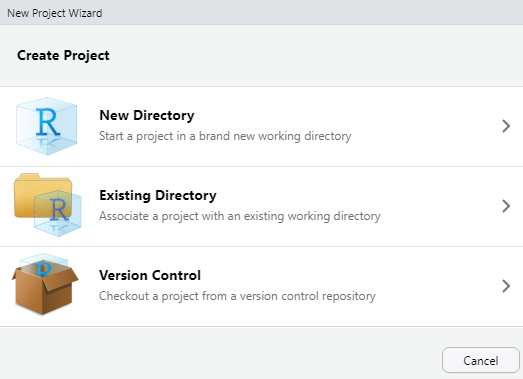
\includegraphics{images/projoption1.png}

Then select ``New project'',

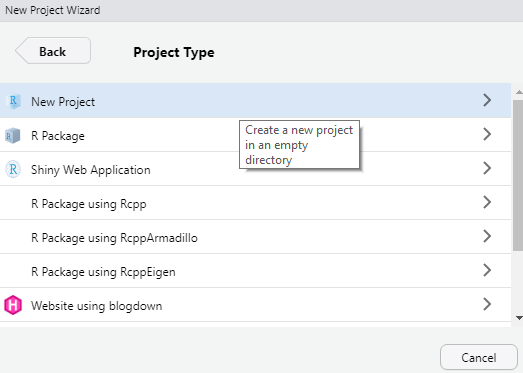
\includegraphics{images/projoption2.png}

enter a name for the project, and browse to where you want the directory located on your computer.

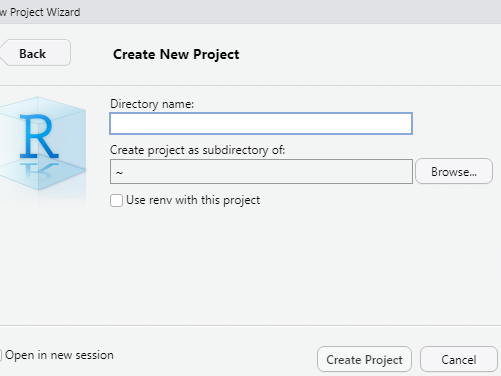
\includegraphics{images/projdirectory.png}

Complete the process by clicking ``Create Project.''

\hypertarget{troubleshooting-3}{%
\subsection{Troubleshooting}\label{troubleshooting-3}}

\begin{itemize}
\tightlist
\item
  You need to know where your project folders are on your computer. I recommend that you create a master folder called ``PSC 253'', and then have all of your project folders inside of that master folder.
\item
  We will use separate projects for each lab assignment and for the Data Project assignment.
\item
  Avoid having multiple project folders for the same assignment. It will cause confusion when you are trying to submit the correct project folder for your assignment.
\end{itemize}

\hypertarget{installpack}{%
\section{Installing a Package}\label{installpack}}

A \emph{package} is a specialized collection of R elements -- datasets, functions, objects, etc. We will use various packages to help in our data analysis. Packages have to be installed and loaded before their elements can be accessed, so this section will teach you how to install a package.

\hypertarget{problem-6}{%
\subsection{Problem}\label{problem-6}}

You want to install a package.

\hypertarget{solution-6}{%
\subsection{Solution}\label{solution-6}}

\begin{enumerate}
\def\labelenumi{\arabic{enumi}.}
\tightlist
\item
  You can type in the command \texttt{install.packages("packagename")}. Thus, to install the package named ``here'' we would type \texttt{install.packages("here")}.
\end{enumerate}

\begin{Shaded}
\begin{Highlighting}[]
\CommentTok{\# installing the RCPA3 package}

\FunctionTok{install.packages}\NormalTok{(}\StringTok{"RCPA3"}\NormalTok{)}
\end{Highlighting}
\end{Shaded}

Alternatively, you can use the menu bar:

\begin{enumerate}
\def\labelenumi{\arabic{enumi}.}
\tightlist
\item
  Click on ``Tools'' in the menu bar.
\item
  select ``Install Packages''
\item
  A dialogue box will appear.
\item
  Type in the name of the package you want.
\item
  Click ``Install''.
\end{enumerate}

\hypertarget{troubleshooting-4}{%
\subsection{Troubleshooting}\label{troubleshooting-4}}

\begin{itemize}
\tightlist
\item
  Some packages depend on the installation of other packages first. R will install these dependencies automatically, so it may take a while for your package to install. You know the installation is done when the console shows its arrow and blinking cursor.
\item
  If you get a message asking you to install Rtools, then you can do so {[}here{]}{[}\url{https://cran.r-project.org/bin/windows/Rtools/}{]}.
\item
  If you get a message that says ``exited with non-zero status'', then the package did not fully install. This could be due to one of the dependency packages not installing properly. Try to install that dependency package manually -- \texttt{install.packages("dependencyname")}. Once the dependent package is installed, you can try to install the main package again.
\item
  You will know that the package has been successfully installed if you are able to load the package.
\item
  In rare occasions, a package may require a later edition of R than you have installed on your computer. The message will say something like ``This package requires R 4.1.0 and you have R 3.1.0''. In that case, you will need to download and install the latest version of R before you can install the package.
\item
  Remember to use quotation marks around the package name in \texttt{install.packages()}.
\end{itemize}

\hypertarget{loadpack}{%
\section{Loading a Package}\label{loadpack}}

It is not enough to just install a package. Installed packages must be loaded in order for you to access their elements.

\hypertarget{problem-7}{%
\subsection{Problem}\label{problem-7}}

You want to load a package that you have installed.

\hypertarget{solution-7}{%
\subsection{Solution}\label{solution-7}}

The function we use to load packages is \texttt{library()}. Its main argument is the name of the package -- \texttt{library(packagename)}.

\begin{Shaded}
\begin{Highlighting}[]
\CommentTok{\# load the RCPA3 package}

\FunctionTok{library}\NormalTok{(RCPA3)}
\end{Highlighting}
\end{Shaded}

\hypertarget{troubleshooting-5}{%
\subsection{Troubleshooting}\label{troubleshooting-5}}

\begin{itemize}
\tightlist
\item
  Packages must be fully and properly installed before they can be loaded.
\item
  If you get an error saying that a package does not exist then 1) you have not installed the package or 2) you have spelled the name of the package incorrectly.
\item
  Remember that we do not put the name of the package in quotation marks when we are loading it.
\end{itemize}

\hypertarget{relative-path}{%
\section{Using relative file paths}\label{relative-path}}

Whenever we load data or save data we will need to specify a file path -- where the file is located on the computer. Obviously, the file path on your computer will not be the same as the path on someone else's computer. We want our code to be able to run on any computer, so we create \emph{relative} file paths. That is, we specify where the file is located relative to the \protect\hyperlink{project}{project folder}.

\hypertarget{problem-8}{%
\subsection{Problem}\label{problem-8}}

You want to create a file path relative to the project folder.

\hypertarget{solution-8}{%
\subsection{Solution}\label{solution-8}}

\begin{enumerate}
\def\labelenumi{\arabic{enumi}.}
\tightlist
\item
  You need to already have a project folder. See Section \ref{project}.
\item
  Load the ``here'' package
\item
  The function \texttt{here()} automatically sets the relative point of the file path as the location of your \texttt{.Rproj} file.
\item
  You can then provide the file path as the argument to \texttt{here()}.
\end{enumerate}

\begin{Shaded}
\begin{Highlighting}[]
\CommentTok{\# Creating a path to the "images" folder in this project.}

\FunctionTok{library}\NormalTok{(here)}
\end{Highlighting}
\end{Shaded}

\begin{verbatim}
## here() starts at E:/OneDrive/R Code/PSC 253 Manual
\end{verbatim}

\begin{Shaded}
\begin{Highlighting}[]
\FunctionTok{here}\NormalTok{(}\StringTok{"images"}\NormalTok{)}
\end{Highlighting}
\end{Shaded}

\begin{verbatim}
## [1] "E:/OneDrive/R Code/PSC 253 Manual/images"
\end{verbatim}

For example, we have a project folder named \texttt{hypothesis\_test\_lab}. Figure \ref{fig:here-example} shows the inside of that project folder. There are three subfolders: Data, Documents, and Scripts. Inside the ``Data'' folder there are two more folders called \texttt{Analysis\_Data} and \texttt{Original\_Data}.

\begin{figure}
\centering
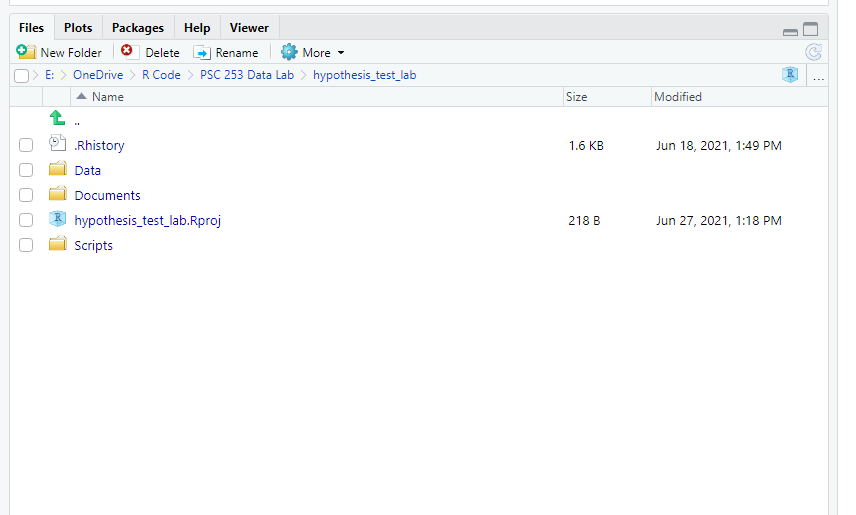
\includegraphics{images/here_example1.png}
\caption{\label{fig:here-example}A screen shot of the hypothesistestlab project folder.}
\end{figure}

We will use the \texttt{here()} function to load a data file that is found within the \texttt{Analysis\_Data} folder.

\begin{Shaded}
\begin{Highlighting}[]
\CommentTok{\# loading "analysis1.RData" file}

\FunctionTok{load}\NormalTok{(}\FunctionTok{here}\NormalTok{(}\StringTok{"Data/Analysis\_Data/analysis1.RData"}\NormalTok{))}
\end{Highlighting}
\end{Shaded}

\hypertarget{troubleshooting-6}{%
\subsection{Troubleshooting}\label{troubleshooting-6}}

\begin{itemize}
\tightlist
\item
  Remember to use forward slashes \texttt{/} and quotation marks when writing the relative path for \texttt{here()}.
\item
  The use of \texttt{here()} is a new function introduced in Fall 2021. Code from prior versions of the course that used relative paths may need to be revised if you want to use the \texttt{here()} function.
\item
  Your first code chunk should load the \texttt{here} package -- \texttt{library(here)}.
\end{itemize}

\hypertarget{csv-load}{%
\section{Loading .csv Data}\label{csv-load}}

There are some packages that come with datasets attached to them. However, we will mostly need to import datasets into R. This section deals with how to specify the file path for the data and the various functions that correspond to the different types of data files you may encounter.

\hypertarget{problem-9}{%
\subsection{Problem}\label{problem-9}}

You want to load a datafile that takes the form \texttt{data\_name.csv}.

\hypertarget{solution-9}{%
\subsection{Solution}\label{solution-9}}

\begin{enumerate}
\def\labelenumi{\arabic{enumi}.}
\tightlist
\item
  You already have a project folder. (Section \ref{project})
\item
  You already know how to create relative paths. (Section \ref{relative-path})
\item
  In this course, \texttt{.csv} files should always be located in the \texttt{Original\_Data} subfolder, which is found inside the ``Data'' folder.
\item
  \protect\hyperlink{object}{Create an object} to hold the data that you will import. This object will be assigned the imported data.
\item
  Use the function \texttt{read.csv()} or \texttt{read\_csv()} to import the data into R. Its argument is the file path.
\end{enumerate}

Generically, the code takes the form:

\begin{Shaded}
\begin{Highlighting}[]
\NormalTok{your\_object }\OtherTok{\textless{}{-}} \FunctionTok{read.csv}\NormalTok{(}\FunctionTok{here}\NormalTok{(}\StringTok{"Data/Original\_Data/your\_data.csv"}\NormalTok{))}
\end{Highlighting}
\end{Shaded}

If I were loading a csv file named ``congbills.csv'' and assigning it to an object called ``bills'', then the code would be:

\begin{Shaded}
\begin{Highlighting}[]
\CommentTok{\# Loading the csv file "congbills.csv" into R as an object called "bills"}

\NormalTok{bills }\OtherTok{\textless{}{-}} \FunctionTok{read.csv}\NormalTok{(}\FunctionTok{here}\NormalTok{(}\StringTok{"Data/Original\_Data/congbills.csv"}\NormalTok{))}
\end{Highlighting}
\end{Shaded}

\hypertarget{troubleshooting-7}{%
\subsection{Troubleshooting}\label{troubleshooting-7}}

\begin{itemize}
\tightlist
\item
  The most common error is that the file path to the data has not been specified properly. Check the spelling in your file path.
\item
  Make sure that you use \texttt{here()} for the file path. Start from the project folder, and then write the path until you get to your file.
\item
  Using \texttt{read\_csv()} requires the \texttt{tidyverse} package.
\end{itemize}

\hypertarget{dta-load}{%
\section{Loading .dta Data}\label{dta-load}}

Stata is another popular software program for data analysis. It is often used in economics. The types of files that are used in Stata have the suffix \texttt{.dta}.

\hypertarget{problem-10}{%
\subsection{Problem}\label{problem-10}}

You want to load a datafile that takes the form \texttt{data\_name.dta}.

\hypertarget{solution-10}{%
\subsection{Solution}\label{solution-10}}

\begin{enumerate}
\def\labelenumi{\arabic{enumi}.}
\tightlist
\item
  You already have a project folder. (Section \ref{project})
\item
  You already know how to create relative paths. (Section \ref{relative-path})
\item
  In this course, \texttt{.dta} files should always be located in the \texttt{Original\_Data} subfolder, which is found inside the ``Data'' folder.
\item
  \protect\hyperlink{object}{Create an object} to hold the data that you will import. This object will be assigned the imported data.
\item
  \protect\hyperlink{loadpack}{Load the package} \texttt{haven} -- \texttt{library(haven)}
\item
  Use the function \texttt{read\_dta()} to import the data into R. Its argument is the file path.
\end{enumerate}

Generically, the code takes the form:

\begin{Shaded}
\begin{Highlighting}[]
\CommentTok{\# load the package \textquotesingle{}haven\textquotesingle{}}
\FunctionTok{library}\NormalTok{(haven)}

\CommentTok{\# import the data}
\NormalTok{your\_object }\OtherTok{\textless{}{-}} \FunctionTok{read\_data}\NormalTok{(}\FunctionTok{here}\NormalTok{(}\StringTok{"Data/Original\_Data/your\_data.dta"}\NormalTok{))}
\end{Highlighting}
\end{Shaded}

If I were loading a dta file named ``congbills.dta'' and assigning it to an object called ``bills'', then the code would be:

\begin{Shaded}
\begin{Highlighting}[]
\CommentTok{\# Loading the dta file "congbills.dta" into R as an object called "bills"}

\NormalTok{bills }\OtherTok{\textless{}{-}} \FunctionTok{read\_dta}\NormalTok{(}\FunctionTok{here}\NormalTok{(}\StringTok{"Data/Original\_Data/congbills.dta"}\NormalTok{))}
\end{Highlighting}
\end{Shaded}

\hypertarget{troubleshooting-8}{%
\subsection{Troubleshooting}\label{troubleshooting-8}}

\begin{itemize}
\tightlist
\item
  The most common error is that the file path to the data has not been specified properly. Check the spelling in your file path.
\item
  Make sure that you use \texttt{here()} for the file path. Start from the project folder, and then write the path until you get to your file.
\item
  Using \texttt{read\_dta()} requires the \texttt{haven} package.
\end{itemize}

\hypertarget{organizing-for-reproducibility}{%
\chapter{Organizing for Reproducibility}\label{organizing-for-reproducibility}}

\hypertarget{tiercreate}{%
\section{Create TIER Folders}\label{tiercreate}}

\hypertarget{problem-11}{%
\subsection{Problem}\label{problem-11}}

You want to create folders in accordance with \href{https://www.projecttier.org/tier-protocol/protocol-4-0/}{Project TIER's protocol}.

\hypertarget{solution-11}{%
\subsection{Solution}\label{solution-11}}

\begin{enumerate}
\def\labelenumi{\arabic{enumi}.}
\tightlist
\item
  You should have already \protect\hyperlink{project}{created a project}.
\end{enumerate}

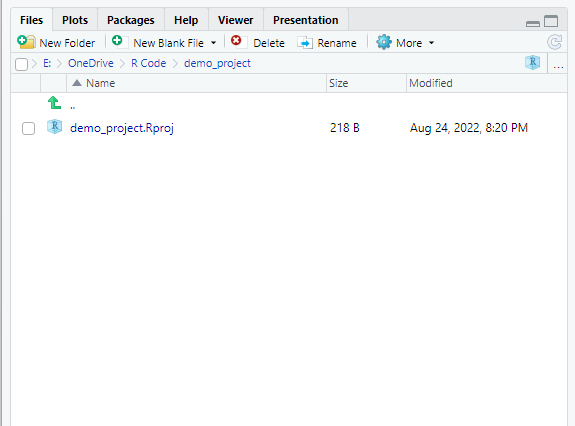
\includegraphics{images/projdirectory2.png}

\begin{enumerate}
\def\labelenumi{\arabic{enumi}.}
\setcounter{enumi}{1}
\tightlist
\item
  In the Files, Plots, Packages, Help, Viewer pane there is a button that says ``New Folder.''
\end{enumerate}

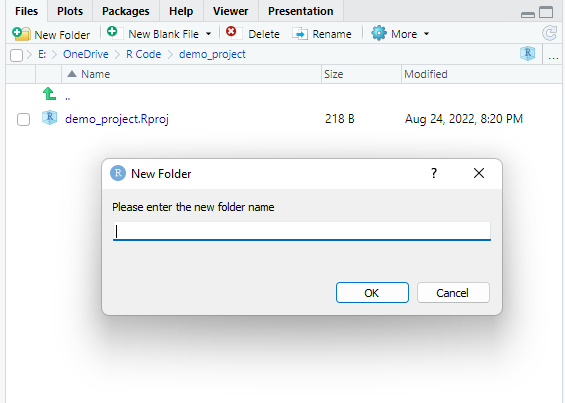
\includegraphics{images/newfolder.png}

\begin{enumerate}
\def\labelenumi{\arabic{enumi}.}
\setcounter{enumi}{2}
\tightlist
\item
  Click that button to create three folders named ``Data'', ``Documents'', and ``Script''. When you are finished the project folder should look like this:
\end{enumerate}

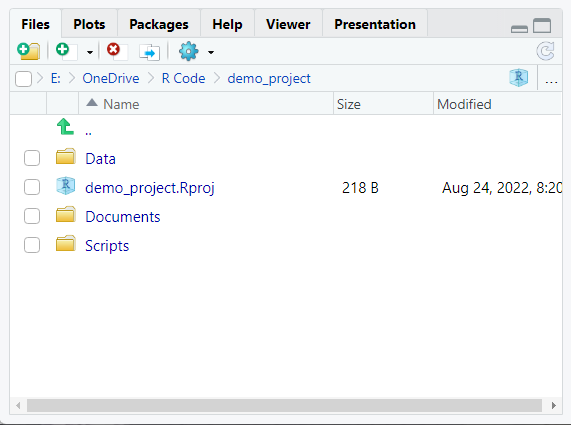
\includegraphics{images/tiermain.png}

\begin{enumerate}
\def\labelenumi{\arabic{enumi}.}
\setcounter{enumi}{3}
\tightlist
\item
  Inside the ``Data'' folder, create two folders named ``Input\_Data'' and ``Analysis\_Data''.
\end{enumerate}

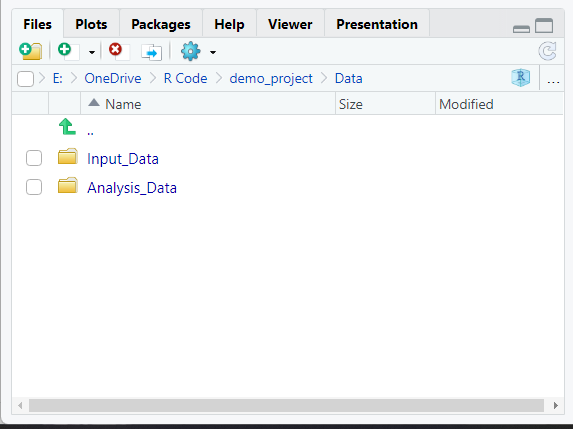
\includegraphics{images/tierdata.png}

\begin{enumerate}
\def\labelenumi{\arabic{enumi}.}
\setcounter{enumi}{4}
\tightlist
\item
  Inside the ``Scripts'' folder, create three folders named ``Processing'', ``Data\_Appendix'', and ``Analysis''.
\end{enumerate}

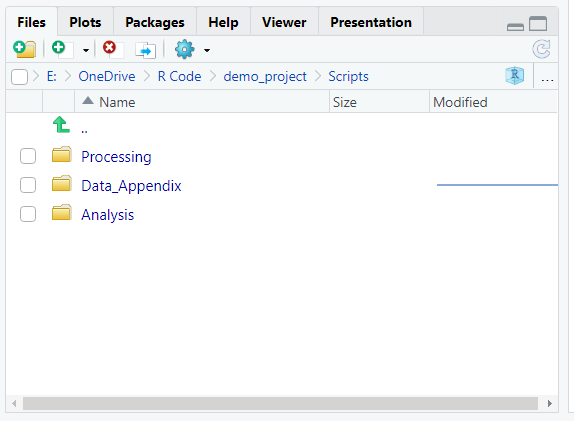
\includegraphics{images/tierscripts.png}

\hypertarget{troubleshooting-9}{%
\subsection{Troubleshooting}\label{troubleshooting-9}}

\begin{itemize}
\tightlist
\item
  The actual names of the folder are not important. However, you should be consistent with how you name the folders across projects. That will help you to remember the role that each folder serves.
\item
  Keep in mind that you will use these folder names in your \protect\hyperlink{relative-path}{relative paths}.
\end{itemize}

\hypertarget{tierpopulate}{%
\section{Populate TIER Folders}\label{tierpopulate}}

\hypertarget{problem-12}{%
\subsection{Problem}\label{problem-12}}

You want to put files into their appropriate TIER folder.

\hypertarget{solution-12}{%
\subsection{Solution}\label{solution-12}}

\begin{enumerate}
\def\labelenumi{\arabic{enumi}.}
\tightlist
\item
  You have already \protect\hyperlink{project}{created a project folder}.
\item
  You have already \protect\hyperlink{tiercreate}{created TIER folders} inside of the project folder.
\item
  Now we are ready to describe what goes into each of these folders. We will start with the ``Data'' folder.
\end{enumerate}

Inside of the ``Data'' folder there are two subfolders -- ``Input\_Data'' and ``Analysis Data''. The ``Input\_Data'' folder is where you place the unprocessed, original version of a dataset. Also, you should create a subfolder inside of the ``Input\_Data'' folder that is called ``Metadata''. Any codebooks that are associated with your dataset should be placed inside of the ``Metadata'' folder.

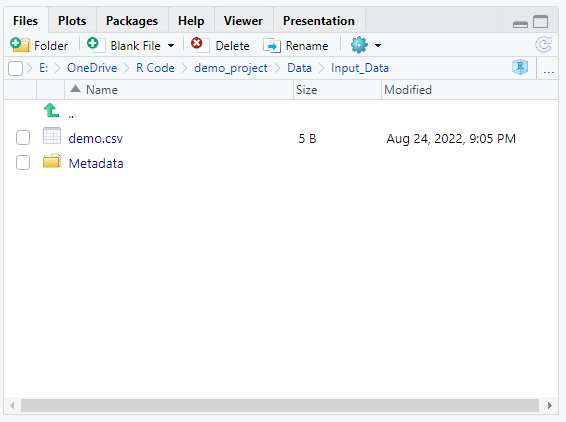
\includegraphics{images/tierinput.png}

You do not place anything inside of the ``Analysis\_Data'' folder. This folder will be populated when the input data is processed.

\begin{enumerate}
\def\labelenumi{\arabic{enumi}.}
\setcounter{enumi}{3}
\tightlist
\item
  Inside of the ``Scripts'' folder there are three subfolders -- ``Processing'', ``Analysis'', and ``Data\_Appendix''. The ``Processing'' folder should have one file named \texttt{processing.rmd}. This file is used to transform the input data into the form that you will use for the data analysis.
\end{enumerate}

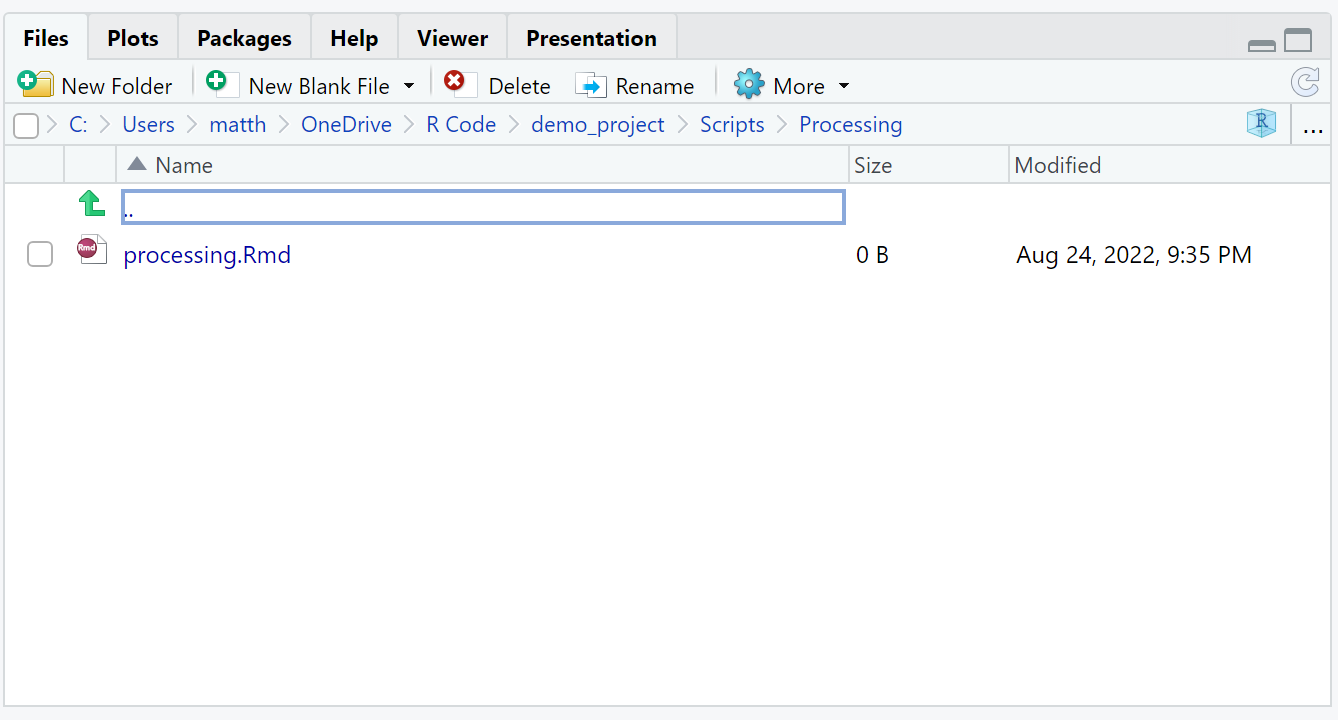
\includegraphics{images/tierprocessing.png}

The ``Data\_Appendix'' folder should have one filed named \texttt{data-appendix.rmd}. This file creates the Data Appendix, which serves as a codebook and provides descriptive statistics for the variables that are used in the actual data analysis.

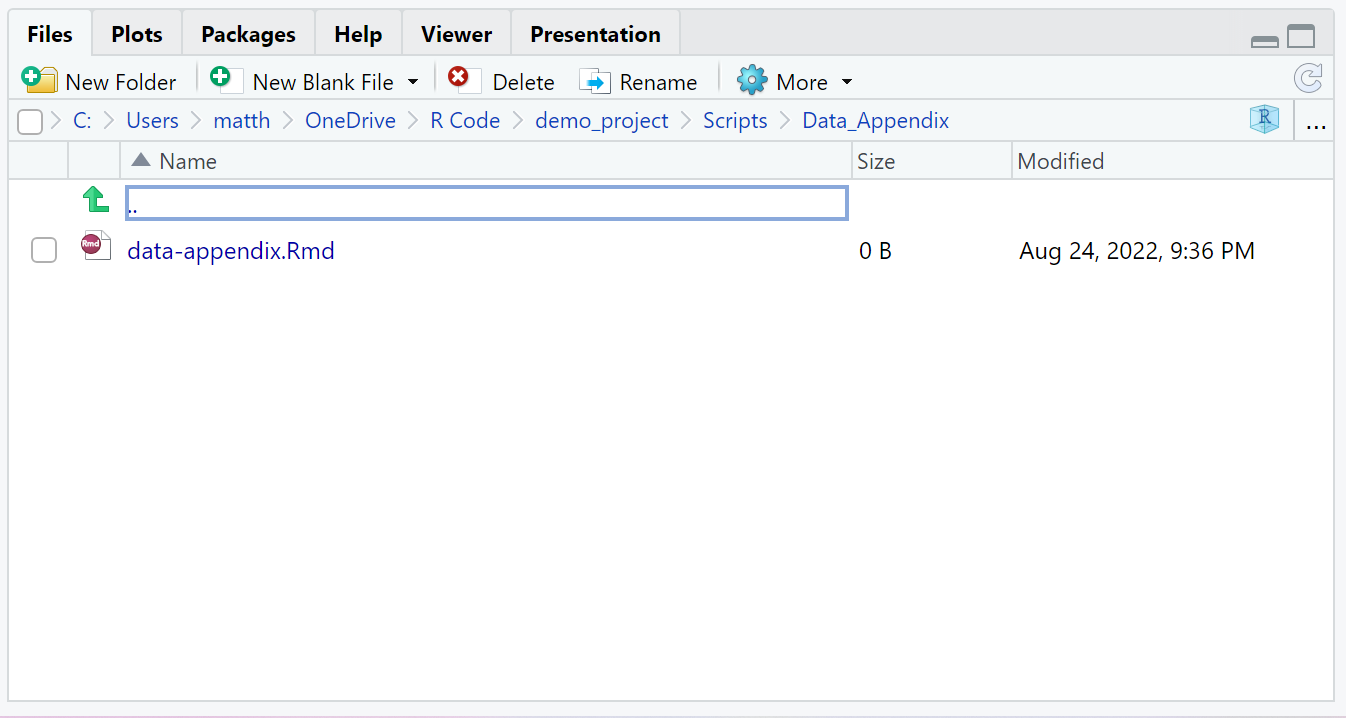
\includegraphics{images/data-appendix.png}

Lastly, the ``Analysis'' folder should have one file named \texttt{analysis.rmd}. For the final data project, this file will contain all of the data analysis that you were required to perform as part of that project. For the weekly labs, the \texttt{analysis.rmd} provides sample code for any analysis that you will be required to perform in the lab report.

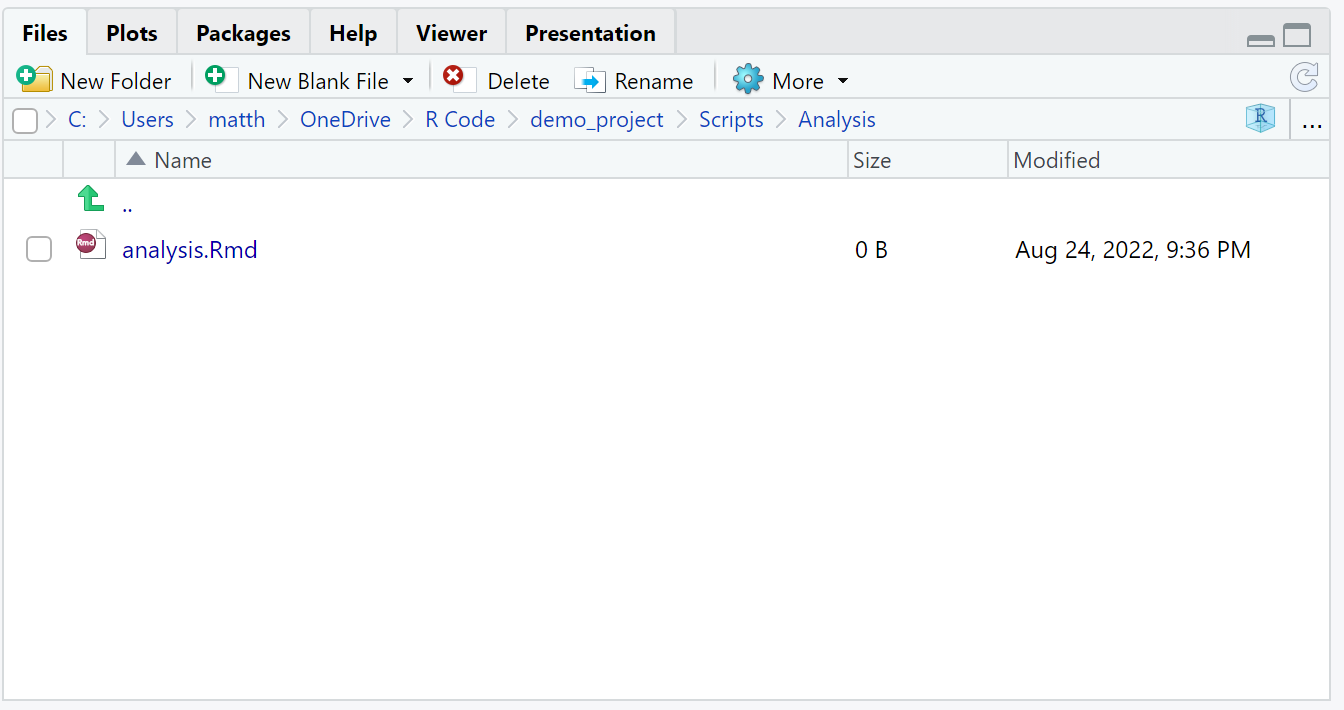
\includegraphics{images/tieranalysis.png}

\begin{enumerate}
\def\labelenumi{\arabic{enumi}.}
\setcounter{enumi}{4}
\tightlist
\item
  The ``Documents'' folder contains the finished version of your work -- the lab report, the research paper, or the final poster. This folder may also contain any supplementary files or folders that are necessary for that final product. For example, files for the Morehouse logo that appears on the final data project poster are located inside of the ``Documents'' folder.
\end{enumerate}

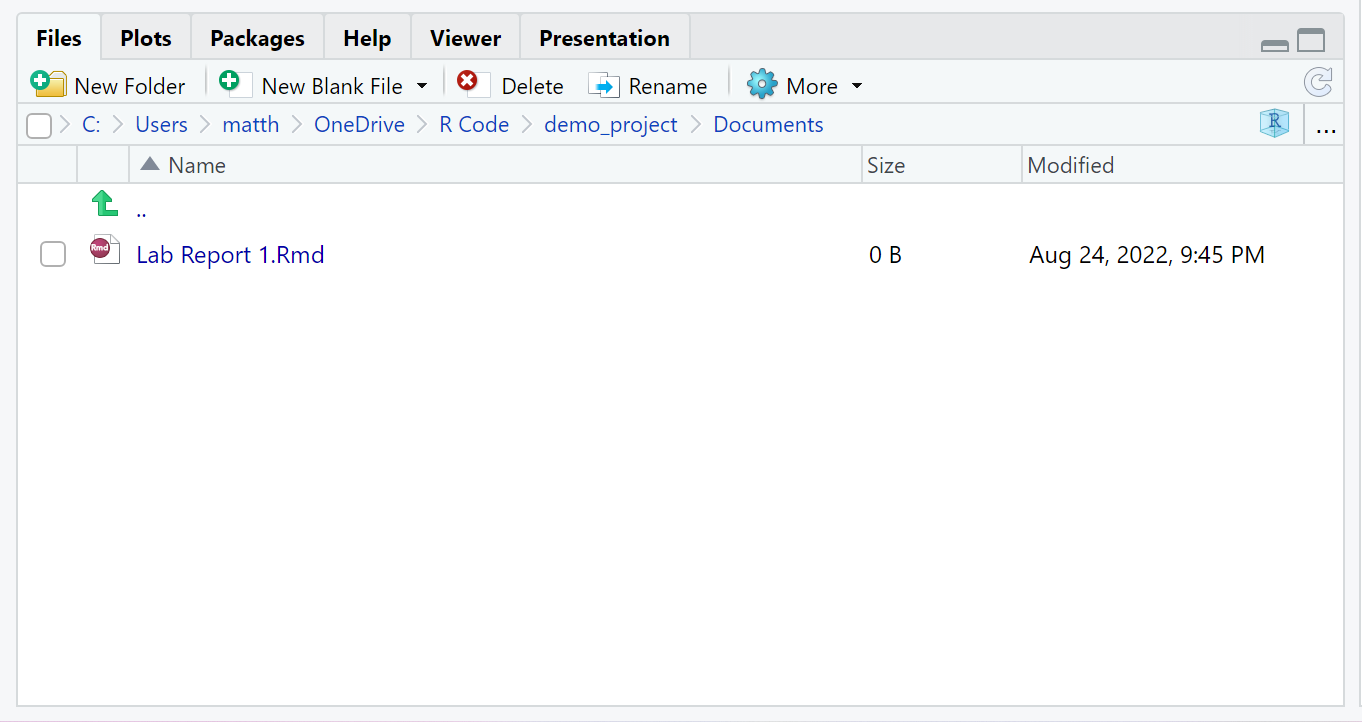
\includegraphics{images/labreport.png}

\hypertarget{troubleshooting-10}{%
\subsection{Troubleshooting}\label{troubleshooting-10}}

\begin{itemize}
\tightlist
\item
  Do not confuse the ``Analysis'' subfolder in ``Scripts'' with the ``Analysis\_Data'' subfolder in ``Data''.
\item
  Keep in mind that the actions described above do not have to take place within Rstudio. You can simply use the Explorer or Finder windows on your computer to achieve the same ends.
\end{itemize}

\hypertarget{sequence}{%
\section{Knitting Files in Sequence}\label{sequence}}

\hypertarget{problem-13}{%
\subsection{Problem}\label{problem-13}}

You want to knit your \texttt{.Rmd} files in correct order to produce the finalized report or paper.

\hypertarget{solution-13}{%
\subsection{Solution}\label{solution-13}}

\begin{enumerate}
\def\labelenumi{\arabic{enumi}.}
\item
  Only the \texttt{processing.Rmd} file should work with your input data, so it is always knit first.
\item
  The processing script creates a file called ``analysis.RData''. This is the analysis data that will be loaded by all of the other scripts.
\item
  Knit the \texttt{data-appendix.Rmd} so that you can become familiar with the variables that you are analyzing.
\item
  Knit the \texttt{analysis.Rmd} third. It will serve as a guide/template to help you complete the lab resort.
\item
  Knit the final report.
\end{enumerate}

\hypertarget{troubleshotting}{%
\subsection{Troubleshotting}\label{troubleshotting}}

\begin{itemize}
\tightlist
\item
  If there is a knitting error about loading data for the analysis or data-appendix script, then check to make sure that you have successfully knitted the processing script. Look in the ``Analysis\_Data'' folder to make sure that the ``analysis.RData'' has been created.
\item
  The relative file paths assume that you are working within the project folder. Look in the top right corner to make sure that it shows that you are working in the appropriate project.
\end{itemize}

\hypertarget{processing-data}{%
\chapter{Processing Data}\label{processing-data}}

Most of the time, we need to make some changes to a dataset to prepare it for analysis. This could involve adding new variables, ``cleaning'' existing variables, changing the level of measurement for a variable, altering the labels of a variable, or even combining multiple datasets. We refer to these kinds of changes as ``processing'' the data. This section is about the common tools that are used for data processing in this course.

\hypertarget{missing}{%
\section{Label Missing Observations in a Dataset}\label{missing}}

Sometimes we will work with survey data that has observations with numeric codes that are not aligned with a response of interest. For example, the numeric code -9 might signify that a person did not actually answer the survey question. We want to label this particular observation as ``missing''.

\hypertarget{problem-14}{%
\subsection{Problem}\label{problem-14}}

You want to label missing observations.

\hypertarget{solution-14}{%
\subsection{Solution}\label{solution-14}}

\begin{enumerate}
\def\labelenumi{\arabic{enumi}.}
\tightlist
\item
  These instructions begin with the premise that you already know which variable values correspond to missing values.The codebook should indicate which codes correspond to missing data.
\item
  Use indexing to isolate the observations that have missing values.
\item
  Assign those observations a value of \texttt{NA}.
\end{enumerate}

\begin{Shaded}
\begin{Highlighting}[]
\NormalTok{dataset}\SpecialCharTok{$}\NormalTok{variable[dataset}\SpecialCharTok{$}\NormalTok{variable }\SpecialCharTok{==}\NormalTok{ missing\_value] }\OtherTok{\textless{}{-}} \ConstantTok{NA}
\end{Highlighting}
\end{Shaded}

Here we are looking at the variable \texttt{hillary\_therm} in the \texttt{anes} dataset, and we label all observations that take the value -9 as missing.

\begin{Shaded}
\begin{Highlighting}[]
\CommentTok{\# labeling {-}9 as missing}
\NormalTok{anes}\SpecialCharTok{$}\NormalTok{hillary\_therm[anes}\SpecialCharTok{$}\NormalTok{hillary\_therm }\SpecialCharTok{==} \SpecialCharTok{{-}}\DecValTok{9}\NormalTok{] }\OtherTok{\textless{}{-}} \ConstantTok{NA}
\end{Highlighting}
\end{Shaded}

\hypertarget{troubleshooting-11}{%
\subsection{Troubleshooting}\label{troubleshooting-11}}

\begin{itemize}
\tightlist
\item
  In order to label the missing observations you have to first understand what all of the values of the variable are and/or should be. That information comes from the codebook for the data. For example, if you know that a variable is supposed to take values from 0 to 10, then a value of -99 is probably a code for a missing observation.
\item
  You will generally want to look at a frequency table prior to labeling the missing values and after labeling the missing values. That will indicate whether you have done it correctly.
\end{itemize}

\hypertarget{add-variable}{%
\section{Add a New Variable to a Dataset}\label{add-variable}}

When we want to make a change to a variable, it is a good practice to create a new variable rather than changing the existing variable.

\hypertarget{problem-15}{%
\subsection{Problem}\label{problem-15}}

You want to add a variable to a dataset.

\hypertarget{solution---basic}{%
\subsection{Solution - Basic}\label{solution---basic}}

\begin{enumerate}
\def\labelenumi{\arabic{enumi}.}
\tightlist
\item
  Provide a name for the new variable.
\item
  Use the \texttt{\$} operator to create the variable in the data \texttt{data\$new\_variable\_name}.
\item
  Assign values to the new variable. Often we are assigning the new variable the values of the old variable as a preliminary step to some other kind of transformation/processing. \texttt{data\$new\_variable\ \textless{}-\ data\$old\_variable}.
\end{enumerate}

\begin{Shaded}
\begin{Highlighting}[]
\CommentTok{\# assign an old variable to a new variable name}
\NormalTok{dataset}\SpecialCharTok{$}\NormalTok{new\_variable }\OtherTok{\textless{}{-}}\NormalTok{ dataset}\SpecialCharTok{$}\NormalTok{old\_variable}
\end{Highlighting}
\end{Shaded}

Below we assign the values of the variable \texttt{ft.dem} to a new variable called \texttt{dem\_therm}. The dataset is named ``nes''.

\begin{Shaded}
\begin{Highlighting}[]
\NormalTok{nes}\SpecialCharTok{$}\NormalTok{dem\_therm }\OtherTok{\textless{}{-}}\NormalTok{ nes}\SpecialCharTok{$}\NormalTok{ft.dem}
\end{Highlighting}
\end{Shaded}

\hypertarget{solution---tidyverse}{%
\subsection{Solution - tidyverse}\label{solution---tidyverse}}

\begin{enumerate}
\def\labelenumi{\arabic{enumi}.}
\tightlist
\item
  Assign the dataset to itself.
\item
  Use the pipe operator \texttt{\%\textgreater{}\%} at the end of that line of code.
\item
  Use the \texttt{mutate()} function.
\item
  The argument for the function is setting the name of the new variable and then assigning it values using an equal sign.
\end{enumerate}

\begin{Shaded}
\begin{Highlighting}[]
\CommentTok{\# use mutate to turn an old variable into a new variable}

\NormalTok{dataset }\OtherTok{\textless{}{-}}\NormalTok{ dataset }\SpecialCharTok{\%\textgreater{}\%}
  \FunctionTok{mutate}\NormalTok{(}\AttributeTok{new\_variable =}\NormalTok{ old\_variable)}
\end{Highlighting}
\end{Shaded}

Below we assign the values of the variable \texttt{ft.dem} to a new variable called \texttt{dem\_therm}. The dataset is named ``nes''.

\begin{Shaded}
\begin{Highlighting}[]
\CommentTok{\# assign data to itself}
\NormalTok{nes }\OtherTok{\textless{}{-}}\NormalTok{ nes }\SpecialCharTok{\%\textgreater{}\%}
  
  \CommentTok{\# use mutate() to assign values to the new variable}
  \FunctionTok{mutate}\NormalTok{(}\AttributeTok{dem\_therm =}\NormalTok{ ft.dem)}
\end{Highlighting}
\end{Shaded}

\hypertarget{troubleshooting-12}{%
\subsection{Troubleshooting}\label{troubleshooting-12}}

\begin{itemize}
\tightlist
\item
  No common mistakes yet.
\end{itemize}

\hypertarget{additive}{%
\section{Create an Additive Index}\label{additive}}

\hypertarget{problem-16}{%
\subsection{Problem}\label{problem-16}}

You want to make some arithmetic adjustment to a variable.

\hypertarget{solution-15}{%
\subsection{Solution}\label{solution-15}}

\begin{enumerate}
\def\labelenumi{\arabic{enumi}.}
\tightlist
\item
  You have already \protect\hyperlink{add-variable}{added a variable to a dataset}
\item
  Inside your \texttt{mutate()} function add, subtract, multiply, or divide variables by other variables or by constants.
\end{enumerate}

\begin{Shaded}
\begin{Highlighting}[]
\CommentTok{\# assign dataset to itself}
\NormalTok{dataset }\OtherTok{\textless{}{-}}\NormalTok{ datasets }\SpecialCharTok{\%\textgreater{}\%}
  
  \CommentTok{\# use mutate() with some arithmetic in the argument}
  \FunctionTok{mutate}\NormalTok{(}\AttributeTok{new\_variable =}\NormalTok{ old\_variable }\SpecialCharTok{+}\NormalTok{ some\_number)}
\end{Highlighting}
\end{Shaded}

Below we create a variable \texttt{avg\_demfeel} that is the average feeling thermometer of \texttt{ft.obama}, \texttt{ft.dem}, and \texttt{ft.biden.pre}.

\begin{Shaded}
\begin{Highlighting}[]
\CommentTok{\# assign dataset to itself}
\NormalTok{nes }\OtherTok{\textless{}{-}}\NormalTok{ nes }\SpecialCharTok{\%\textgreater{}\%}
  
  \CommentTok{\# use mutate() to add the three variables and divide to get the average}
  \FunctionTok{mutate}\NormalTok{(}\AttributeTok{avg\_demfeel =}\NormalTok{ (ft.obama }\SpecialCharTok{+}\NormalTok{ ft.dem }\SpecialCharTok{+}\NormalTok{ ft.biden.pre)}\SpecialCharTok{/}\DecValTok{3}\NormalTok{)}
\end{Highlighting}
\end{Shaded}

\hypertarget{troubleshooting-13}{%
\subsection{Troubleshooting}\label{troubleshooting-13}}

\begin{itemize}
\tightlist
\item
  It may be helpful to test out your math problem first to make sure it gives you the results you are looking for.
\end{itemize}

\hypertarget{factor}{%
\section{Create a Factor Variable}\label{factor}}

In R, nominal level variables are called ``factors.'' This section explains how to create a factor.

\hypertarget{problem-17}{%
\subsection{Problem}\label{problem-17}}

You want to transform a variable into a factor.

\hypertarget{solution-16}{%
\subsection{Solution}\label{solution-16}}

\begin{enumerate}
\def\labelenumi{\arabic{enumi}.}
\tightlist
\item
  Decide on what to name the factor variable.
\item
  Use \texttt{as.factor()} to assign the old variable values to the new variable. See Section \ref{add-variable}.
\item
  Use \texttt{levels()} to assign labels to the values of the variable.
\item
  The levels should be provided as a list in \texttt{c()} with the names of the levels in quotation marks.
\item
  It would follow the general template below.
\end{enumerate}

\begin{Shaded}
\begin{Highlighting}[]
\CommentTok{\# define the variable as a factor}

\NormalTok{data}\SpecialCharTok{$}\NormalTok{newvariable }\OtherTok{\textless{}{-}} \FunctionTok{as.factor}\NormalTok{(data}\SpecialCharTok{$}\NormalTok{oldvariable)}

\CommentTok{\# add the levels}

\FunctionTok{levels}\NormalTok{(data}\SpecialCharTok{$}\NormalTok{newvariable) }\OtherTok{\textless{}{-}} \FunctionTok{c}\NormalTok{(}\StringTok{"label1"}\NormalTok{, }\StringTok{"label2"}\NormalTok{, }\StringTok{"labelk"}\NormalTok{)}
\end{Highlighting}
\end{Shaded}

Transform \texttt{battleground2020} in the \texttt{states} from a numeric dummy variable into a factor.

\begin{Shaded}
\begin{Highlighting}[]
\CommentTok{\# the frequency table for the old variable}
\FunctionTok{freqC}\NormalTok{(states}\SpecialCharTok{$}\NormalTok{battleground2020, }\AttributeTok{plot =}\NormalTok{ F)}
\end{Highlighting}
\end{Shaded}

\begin{verbatim}
## ===========================================================================
##           Describing Distribution of Values with Frequency Table
## ===========================================================================
## 
## 
## Table: \label{tab:unnamed-chunk-44}Frequency Distribution of states$battleground2020 (Battleground in 2020 election? )
## 
##          Frequency   Percent
## ------  ----------  --------
## 0               37     74.00
## 1               13     26.00
## Total           50    100.00
\end{verbatim}

\begin{Shaded}
\begin{Highlighting}[]
\CommentTok{\# call the new variable \textasciigrave{}battlefact\textasciigrave{}}
\NormalTok{states}\SpecialCharTok{$}\NormalTok{battlefact }\OtherTok{\textless{}{-}} \FunctionTok{as.factor}\NormalTok{(states}\SpecialCharTok{$}\NormalTok{battleground2020)}

\CommentTok{\# assign the levels}
\FunctionTok{levels}\NormalTok{(states}\SpecialCharTok{$}\NormalTok{battlefact) }\OtherTok{\textless{}{-}} \FunctionTok{c}\NormalTok{(}\StringTok{"not a battleground"}\NormalTok{, }\StringTok{"battleground"}\NormalTok{)}

\CommentTok{\# the frequency table for the new variable}
\FunctionTok{freqC}\NormalTok{(states}\SpecialCharTok{$}\NormalTok{battlefact, }\AttributeTok{plot =}\NormalTok{ F)}
\end{Highlighting}
\end{Shaded}

\begin{verbatim}
## ===========================================================================
##           Describing Distribution of Values with Frequency Table
## ===========================================================================
## 
## 
## Table: \label{tab:unnamed-chunk-44}Frequency Distribution of states$battlefact
## 
##                       Frequency   Percent
## -------------------  ----------  --------
## not a battleground           37     74.00
## battleground                 13     26.00
## Total                        50    100.00
\end{verbatim}

\hypertarget{troubleshooting-14}{%
\subsection{Troubleshooting}\label{troubleshooting-14}}

\begin{itemize}
\item
  There has to be a level provided for each value of the variable. That is why this process should occur after a variable has been cleaned.
\item
  The level names do not have to be unique. That means this could be used as a (somewhat clunky) method of recoding a variable by collapsing its categories.
\end{itemize}

\hypertarget{numeric}{%
\section{Create a Numeric Variable}\label{numeric}}

Interval level variables are classified as ``numeric''.

\hypertarget{problem-18}{%
\subsection{Problem}\label{problem-18}}

You want to transform an existing variable into a numeric variable.

\hypertarget{solution-17}{%
\subsection{Solution}\label{solution-17}}

\begin{enumerate}
\def\labelenumi{\arabic{enumi}.}
\tightlist
\item
  Decide on what to name the numeric variable. It could be the same name as the old variable.
\item
  Use \texttt{as.numeric()} to assign the old variable values to the new variable.
\item
  It would follow the general template below.
\end{enumerate}

\begin{Shaded}
\begin{Highlighting}[]
\NormalTok{data}\SpecialCharTok{$}\NormalTok{newvariable }\OtherTok{\textless{}{-}} \FunctionTok{as.numeric}\NormalTok{(data}\SpecialCharTok{$}\NormalTok{oldvariable)}
\end{Highlighting}
\end{Shaded}

Here is an example that converts the seven-point party identification scale into a numeric variable.

\begin{Shaded}
\begin{Highlighting}[]
\CommentTok{\# frequency table of the original variable \textasciigrave{}partyid7\textasciigrave{}}
\FunctionTok{freqC}\NormalTok{(nes}\SpecialCharTok{$}\NormalTok{partyid7, }\AttributeTok{plot =}\NormalTok{ F)}
\end{Highlighting}
\end{Shaded}

\begin{verbatim}
## ===========================================================================
##           Describing Distribution of Values with Frequency Table
## ===========================================================================
## 
## 
## Table: \label{tab:unnamed-chunk-46}Frequency Distribution of nes$partyid7 (PRE: SUMMARY: Party ID)
## 
##                                  Frequency   Percent   Cum.Percent
## ------------------------------  ----------  --------  ------------
## 1. Strong Democrat                    1961     23.78         23.78
## 2. Not very strong Democrat            900     10.92         34.70
## 3. Independent-Democrat                975     11.83         46.53
## 4. Independent                         968     11.74         58.27
## 5. Independent-Republican              879     10.66         68.93
## 6. Not very strong Republican          832     10.09         79.02
## 7. Strong Republican                  1730     20.98        100.00
## Total                                 8245    100.00            NA
\end{verbatim}

\begin{Shaded}
\begin{Highlighting}[]
\CommentTok{\# make \textasciigrave{}partyid7\textasciigrave{} numeric}
\NormalTok{nes}\SpecialCharTok{$}\NormalTok{pid7 }\OtherTok{\textless{}{-}} \FunctionTok{as.numeric}\NormalTok{(nes}\SpecialCharTok{$}\NormalTok{partyid7)}

\CommentTok{\# frequency table of the new variable \textasciigrave{}pid7\textasciigrave{}}
\FunctionTok{freqC}\NormalTok{(nes}\SpecialCharTok{$}\NormalTok{pid7, }\AttributeTok{plot =}\NormalTok{ F)}
\end{Highlighting}
\end{Shaded}

\begin{verbatim}
## ===========================================================================
##           Describing Distribution of Values with Frequency Table
## ===========================================================================
## 
## 
## Table: \label{tab:unnamed-chunk-46}Frequency Distribution of nes$pid7
## 
##          Frequency   Percent
## ------  ----------  --------
## 1             1961     23.78
## 2              900     10.92
## 3              975     11.83
## 4              968     11.74
## 5              879     10.66
## 6              832     10.09
## 7             1730     20.98
## Total         8245    100.00
\end{verbatim}

\hypertarget{troubleshooting-15}{%
\subsection{Troubleshooting}\label{troubleshooting-15}}

\begin{itemize}
\tightlist
\item
  Have not come across any problems yet.
\end{itemize}

\hypertarget{ordinal}{%
\section{Create an Ordinal Variable}\label{ordinal}}

\hypertarget{problem-19}{%
\subsection{Problem}\label{problem-19}}

You want to transform an existing variable into an ordinal variable.

\hypertarget{solution-18}{%
\subsection{Solution}\label{solution-18}}

\begin{enumerate}
\def\labelenumi{\arabic{enumi}.}
\tightlist
\item
  Decide on what to name the ordinal variable. It could be the same name as the old variable. However, this could become confusing in your code.
\item
  Use \texttt{as.ordered()} to assign the old variable values to the new variable.
\item
  Use \texttt{levels()} to assign labels to the values of the variable.
\item
  The levels should be provided as a list in \texttt{c()} with the names of the levels in quotation marks.
\item
  It would follow the general template below.
\end{enumerate}

\begin{Shaded}
\begin{Highlighting}[]
\CommentTok{\# define the variable as ordinal}

\NormalTok{data}\SpecialCharTok{$}\NormalTok{newvariable }\OtherTok{\textless{}{-}} \FunctionTok{as.ordered}\NormalTok{(data}\SpecialCharTok{$}\NormalTok{oldvariable)}

\CommentTok{\# add the levels}

\FunctionTok{levels}\NormalTok{(data}\SpecialCharTok{$}\NormalTok{newvariable) }\OtherTok{\textless{}{-}} \FunctionTok{c}\NormalTok{(}\StringTok{"label1"}\NormalTok{, }\StringTok{"label2"}\NormalTok{, }\StringTok{"labelk"}\NormalTok{)}
\end{Highlighting}
\end{Shaded}

Transform \texttt{abort4} in the \texttt{nes} from a factor into an ordinal variable.

\begin{Shaded}
\begin{Highlighting}[]
\CommentTok{\# the frequency table for the old variable}
\FunctionTok{freqC}\NormalTok{(nes}\SpecialCharTok{$}\NormalTok{abort4, }\AttributeTok{plot =}\NormalTok{ F)}
\end{Highlighting}
\end{Shaded}

\begin{verbatim}
## ===========================================================================
##           Describing Distribution of Values with Frequency Table
## ===========================================================================
## 
## 
## Table: \label{tab:unnamed-chunk-48}Frequency Distribution of nes$abort4
## 
##                                 Frequency   Percent
## -----------------------------  ----------  --------
## never                                 870     11.01
## rape, incest, life of mother         1916     24.25
## yes with limits                      1097     13.89
## always                               4017     50.85
## Total                                7900    100.00
\end{verbatim}

\begin{Shaded}
\begin{Highlighting}[]
\CommentTok{\# call the new variable \textasciigrave{}abort4\textasciigrave{}}
\NormalTok{nes}\SpecialCharTok{$}\NormalTok{abort4 }\OtherTok{\textless{}{-}} \FunctionTok{as.ordered}\NormalTok{(nes}\SpecialCharTok{$}\NormalTok{abort4)}

\CommentTok{\# assign the levels}
\FunctionTok{levels}\NormalTok{(nes}\SpecialCharTok{$}\NormalTok{abort4) }\OtherTok{\textless{}{-}} \FunctionTok{c}\NormalTok{(}\StringTok{"never"}\NormalTok{, }\StringTok{"some conditions"}\NormalTok{, }\StringTok{"more conditions"}\NormalTok{, }\StringTok{"always"}\NormalTok{)}

\CommentTok{\# the frequency table for the new variable}
\FunctionTok{freqC}\NormalTok{(nes}\SpecialCharTok{$}\NormalTok{abort4, }\AttributeTok{plot =}\NormalTok{ F)}
\end{Highlighting}
\end{Shaded}

\begin{verbatim}
## ===========================================================================
##           Describing Distribution of Values with Frequency Table
## ===========================================================================
## 
## 
## Table: \label{tab:unnamed-chunk-48}Frequency Distribution of nes$abort4
## 
##                    Frequency   Percent   Cum.Percent
## ----------------  ----------  --------  ------------
## never                    870     11.01         11.01
## some conditions         1916     24.25         35.27
## more conditions         1097     13.89         49.15
## always                  4017     50.85        100.00
## Total                   7900    100.00            NA
\end{verbatim}

\hypertarget{troubleshooting-16}{%
\subsection{Troubleshooting}\label{troubleshooting-16}}

\begin{itemize}
\tightlist
\item
  There has to be a level provided for each value of the variable. That is why this process should occur after a variable has been cleaned.
\item
  The key reason for treating a variable as ordinal rather than nominal in R is to calculate the ``cumulative percent'' column in a frequency table.
\end{itemize}

\hypertarget{indicator}{%
\section{Create an Indicator/Dummy Variable}\label{indicator}}

An indicator variable (also known as a dummy variable) is a conversion of an existing variable such that it takes the value of 1 when the existing variable meets some criteria and the value of 0 otherwise. For example, if we want to plot the proportion of observations who voted for Joe Biden in 2020, then we would first make an indicator variable out of the nominal variable \texttt{presvote2020}.

\hypertarget{problem-20}{%
\subsection{Problem}\label{problem-20}}

You want to create an indicator/dummy variable.

\hypertarget{solution-19}{%
\subsection{Solution}\label{solution-19}}

\begin{enumerate}
\def\labelenumi{\arabic{enumi}.}
\tightlist
\item
  Assign the dataset to itself.
\item
  Use the pipe operator \texttt{\textbar{}\textgreater{}} at the end of that line of code.
\item
  Use the \texttt{mutate()} function.
\item
  Create a name for the indicator variable.
\item
  Set the indicator variable as being equal to a numeric version of whether the old variable satisfies some criteria.
\end{enumerate}

\begin{Shaded}
\begin{Highlighting}[]
\CommentTok{\# assign the dataset to itself}
\NormalTok{dataset }\OtherTok{\textless{}{-}}\NormalTok{ dataset }\SpecialCharTok{|\textgreater{}}
  
  \CommentTok{\# use mutate() to create the indicator variable}
  \FunctionTok{mutate}\NormalTok{(}\AttributeTok{indicator\_variable =} \FunctionTok{as.numeric}\NormalTok{(some\_criteria))}
\end{Highlighting}
\end{Shaded}

Here we create an indicator variable called \texttt{biden\_vote} that takes a value of 1 for all observations in which \texttt{presvote2020} was equal to Joe Biden.

\begin{Shaded}
\begin{Highlighting}[]
\CommentTok{\# assign the dataset to itself}
\NormalTok{nes }\OtherTok{\textless{}{-}}\NormalTok{ nes }\SpecialCharTok{|\textgreater{}}

  \CommentTok{\#use mutate() to create the indicator variable}
  \FunctionTok{mutate}\NormalTok{(}\AttributeTok{biden\_vote =} \FunctionTok{as.numeric}\NormalTok{(presvote2020 }\SpecialCharTok{==} \StringTok{"1. Joe Biden"}\NormalTok{))}

\CommentTok{\# check the new variable}
\FunctionTok{freqC}\NormalTok{(nes}\SpecialCharTok{$}\NormalTok{biden\_vote, }\AttributeTok{plot =}\NormalTok{ F)}
\end{Highlighting}
\end{Shaded}

\begin{verbatim}
## ===========================================================================
##           Describing Distribution of Values with Frequency Table
## ===========================================================================
## 
## 
## Table: \label{tab:unnamed-chunk-50}Frequency Distribution of nes$biden_vote
## 
##          Frequency   Percent
## ------  ----------  --------
## 0             2740     43.65
## 1             3537     56.35
## Total         6277    100.00
\end{verbatim}

\hypertarget{troubleshooting-17}{%
\subsection{Troubleshooting}\label{troubleshooting-17}}

\begin{itemize}
\tightlist
\item
  The criteria is written as variable, logical operator, and value of the variable.
\item
  The values of categorical variables must be in quotation marks.
\item
  The most common error is that the value of the old variable is not written correctly. If the above example did not include the ``1.'' in front of ``Joe Biden'', then the indicator variable would have returned values of 0 for all of the observations.
\end{itemize}

\hypertarget{filter}{%
\section{Filter your Data}\label{filter}}

\hypertarget{problem-21}{%
\subsection{Problem}\label{problem-21}}

You want to create a subset of your data based on some criteria.

\hypertarget{solution-20}{%
\subsection{Solution}\label{solution-20}}

\begin{enumerate}
\def\labelenumi{\arabic{enumi}.}
\tightlist
\item
  Provide a name for the subset of data you are creating.
\item
  Assign the existing dataset to the new data object.
\item
  Use the pipe \texttt{\%\textgreater{}\%}.
\item
  Use \texttt{filter()}. The pipe inherits the dataset from the prior step, so the only argument is the criteria for the subset.
\item
  The criteria use relational logic:
\end{enumerate}

\begin{itemize}
\tightlist
\item
  \texttt{==} equal to
\item
  \texttt{\textgreater{}} greater than
\item
  \texttt{\textless{}} less than
\item
  \texttt{\textgreater{}=} greater than or equal to
\item
  \texttt{\textless{}=} less than or equal to
\item
  \texttt{!=} not equal to
\item
  \texttt{\textbar{}} or, if there are multiple criteria
\item
  \texttt{\&} and, if there are multiple criteria
\end{itemize}

\begin{enumerate}
\def\labelenumi{\arabic{enumi}.}
\tightlist
\item
  Follow the template below.
\end{enumerate}

\begin{Shaded}
\begin{Highlighting}[]
\NormalTok{newdata }\OtherTok{\textless{}{-}}\NormalTok{ old\_data }\SpecialCharTok{\%\textgreater{}\%}
  \FunctionTok{filter}\NormalTok{(criteria)}
\end{Highlighting}
\end{Shaded}

Here we create a subset that only includes people who voted for Biden

\begin{Shaded}
\begin{Highlighting}[]
\CommentTok{\# frequency of \textasciigrave{}biden\_vote\textasciigrave{} in full dataset}
\FunctionTok{freqC}\NormalTok{(nes}\SpecialCharTok{$}\NormalTok{biden\_vote, }\AttributeTok{plot =}\NormalTok{ F)}
\end{Highlighting}
\end{Shaded}

\begin{verbatim}
## ===========================================================================
##           Describing Distribution of Values with Frequency Table
## ===========================================================================
## 
## 
## Table: \label{tab:unnamed-chunk-52}Frequency Distribution of nes$biden_vote
## 
##          Frequency   Percent
## ------  ----------  --------
## 0             2740     43.65
## 1             3537     56.35
## Total         6277    100.00
\end{verbatim}

\begin{Shaded}
\begin{Highlighting}[]
\CommentTok{\# create a subset of \textasciigrave{}nes\textasciigrave{} data that only includes Biden voters}
\NormalTok{bidenites }\OtherTok{\textless{}{-}}\NormalTok{ nes }\SpecialCharTok{\%\textgreater{}\%}
  \FunctionTok{filter}\NormalTok{(biden\_vote }\SpecialCharTok{==} \DecValTok{1}\NormalTok{)}

\CommentTok{\# frequency of a \textasciigrave{}biden\_vote\textasciigrave{} in subset}
\FunctionTok{freqC}\NormalTok{(bidenites}\SpecialCharTok{$}\NormalTok{biden\_vote, }\AttributeTok{plot =}\NormalTok{ F)}
\end{Highlighting}
\end{Shaded}

\begin{verbatim}
## ===========================================================================
##           Describing Distribution of Values with Frequency Table
## ===========================================================================
## 
## 
## Table: \label{tab:unnamed-chunk-52}Frequency Distribution of bidenites$biden_vote
## 
##          Frequency   Percent
## ------  ----------  --------
## 1             3537    100.00
## Total         3537    100.00
\end{verbatim}

\hypertarget{troubleshooting-18}{%
\subsection{Troubleshooting}\label{troubleshooting-18}}

\begin{itemize}
\tightlist
\item
  The criteria is written as variable, logical operator, and value of the variable.
\item
  The values of categorical variables must be in quotation marks.
\end{itemize}

\hypertarget{sum}{%
\section{Summarize Data Using Means}\label{sum}}

\hypertarget{problem-22}{%
\subsection{Problem}\label{problem-22}}

You want to make a summary dataset that shows the mean of one variable for each value of some other variable.

\hypertarget{solution-21}{%
\subsection{Solution}\label{solution-21}}

\begin{enumerate}
\def\labelenumi{\arabic{enumi}.}
\tightlist
\item
  Assign the old data to a new data object.
\item
  Use the pipe \texttt{\%\textgreater{}\%} at the end of the line of code.
\item
  Use \texttt{group\_by()}. The argument is the variable that you want to use to find the means of some other variable.
\item
  Use the pipe \texttt{\%\textgreater{}\%} at the end of the line of code.
\item
  Use \texttt{summarise()}.
\item
  Create a name for the summary variable.
\item
  Set the summary variable as being equal to the mean of the variable that you want to take the mean of.
\end{enumerate}

\begin{Shaded}
\begin{Highlighting}[]
\NormalTok{newdata }\OtherTok{\textless{}{-}}\NormalTok{ old\_data }\SpecialCharTok{\%\textgreater{}\%}
  \FunctionTok{group\_by}\NormalTok{(group\_variable) }\SpecialCharTok{\%\textgreater{}\%}
  \FunctionTok{summarise}\NormalTok{(}\AttributeTok{summary\_variable =} \FunctionTok{mean}\NormalTok{(mean\_variable))}
\end{Highlighting}
\end{Shaded}

Here we calculate the mean feelings towards Obama, \texttt{ft.obama}, by party identification, \texttt{partyid7}.

\begin{Shaded}
\begin{Highlighting}[]
\CommentTok{\# assign old data to a new data object}
\NormalTok{partymeans }\OtherTok{\textless{}{-}}\NormalTok{ nes }\SpecialCharTok{\%\textgreater{}\%}
  
  \CommentTok{\# use group\_by() to group the data by partyid7}
  \FunctionTok{group\_by}\NormalTok{(partyid7) }\SpecialCharTok{\%\textgreater{}\%}
  
  \CommentTok{\# calculate the means of ft.obama}
  \FunctionTok{summarise}\NormalTok{(}\AttributeTok{average =} \FunctionTok{wtd.mean}\NormalTok{(ft.obama, }\AttributeTok{na.rm =}\NormalTok{ T,}
                               \AttributeTok{w =}\NormalTok{ wt))}

\CommentTok{\# show the summary dataset}
\NormalTok{partymeans}
\end{Highlighting}
\end{Shaded}

\begin{verbatim}
## # A tibble: 8 x 2
##   partyid7                      average
##   <ord>                           <dbl>
## 1 1. Strong Democrat               93.3
## 2 2. Not very strong Democrat      83.0
## 3 3. Independent-Democrat          82.0
## 4 4. Independent                   63.0
## 5 5. Independent-Republican        37.7
## 6 6. Not very strong Republican    44.2
## 7 7. Strong Republican             18.4
## 8 <NA>                             77.9
\end{verbatim}

\hypertarget{troubleshooting-19}{%
\subsection{Troubleshooting}\label{troubleshooting-19}}

\begin{itemize}
\tightlist
\item
  For survey data use \texttt{wtd.mean()}. Use \texttt{mean()} for non-survey data.
\end{itemize}

\hypertarget{transform_nom}{%
\section{Transform an interval variable into a nominal variable}\label{transform_nom}}

Many of the tools we use to analyze the relationship between two variables require that the independent variable is nominal or ordinal. In those cases, it can be useful to transform an interval independent variable into a nominal or ordinal version.

\hypertarget{problem-23}{%
\subsection{Problem}\label{problem-23}}

You want to transform an interval variable into a nominal variable.

\hypertarget{solution-22}{%
\subsection{Solution}\label{solution-22}}

\begin{enumerate}
\def\labelenumi{\arabic{enumi}.}
\tightlist
\item
  Assign the dataset to itself.
\item
  Use the pipe operator \texttt{\textbar{}\textgreater{}} at the end of that line of code.
\item
  Use the \texttt{mutate()} function.
\item
  Create a name for the new nominal variable.
\item
  Set the nominal variable as being equal to a \texttt{factor()} of whether the old variable is greater than some value. The choice of value is up to the researcher, but it should make sense as a way to divide the original variable between ``high'' and ``low''.
\item
  Place a comma at the end of your criteria, and press return.
\item
  Use the argument \texttt{labels\ =} to assign levels to the values of the variable.
\item
  The levels should be provided as a list in \texttt{c()} with the names of the levels in quotation marks.
\end{enumerate}

\begin{Shaded}
\begin{Highlighting}[]
\CommentTok{\# assign the dataset to itself}
\NormalTok{dataset }\OtherTok{\textless{}{-}}\NormalTok{ dataset }\SpecialCharTok{|\textgreater{}}
  
  \CommentTok{\# use mutate to create the nominal variable}
  \FunctionTok{mutate}\NormalTok{(}\AttributeTok{new\_nominal =} \FunctionTok{factor}\NormalTok{(}
    
    \CommentTok{\# the criteria for determining high vs. low values}
\NormalTok{    old\_interval }\SpecialCharTok{\textgreater{}}\NormalTok{ some\_value,}
    
    \CommentTok{\# assign the levels to the new variable}
    \AttributeTok{labels =} \FunctionTok{c}\NormalTok{(}\StringTok{"low"}\NormalTok{, }\StringTok{"high"}\NormalTok{)))}
\end{Highlighting}
\end{Shaded}

In the example below we transform the Obama feeling thermometer, \texttt{ft.obama}, into a nominal variable, \texttt{high\_obama}. The interval variable \texttt{ft.obama} ranges from 0 to 100, so we set 60 and above as the value for ``high''.

\begin{Shaded}
\begin{Highlighting}[]
\NormalTok{nes }\OtherTok{\textless{}{-}}\NormalTok{ nes }\SpecialCharTok{|\textgreater{}}
  \FunctionTok{mutate}\NormalTok{(}\AttributeTok{high\_obama =} \FunctionTok{factor}\NormalTok{(ft.obama }\SpecialCharTok{\textgreater{}} \DecValTok{60}\NormalTok{,}
                             \AttributeTok{labels =} \FunctionTok{c}\NormalTok{(}\StringTok{"cool Obama feelings"}\NormalTok{,}
                                        \StringTok{"warm Obama feelings"}\NormalTok{)))}
\FunctionTok{freqC}\NormalTok{(nes}\SpecialCharTok{$}\NormalTok{high\_obama, }\AttributeTok{plot =}\NormalTok{ F)}
\end{Highlighting}
\end{Shaded}

\begin{verbatim}
## ===========================================================================
##           Describing Distribution of Values with Frequency Table
## ===========================================================================
## 
## 
## Table: \label{tab:unnamed-chunk-56}Frequency Distribution of nes$high_obama
## 
##                        Frequency   Percent
## --------------------  ----------  --------
## cool Obama feelings         3653     44.74
## warm Obama feelings         4512     55.26
## Total                       8165    100.00
\end{verbatim}

\hypertarget{troubleshooting-20}{%
\subsection{Troubleshooting}\label{troubleshooting-20}}

\begin{itemize}
\tightlist
\item
  Make sure that you have the correct number of closing parentheses. Following the template above, there should be three parentheses at the end.
\item
  Remember that we are converting an interval variable, so the value of that variable should be a number without quotation marks.
\end{itemize}

\hypertarget{transform_ord}{%
\section{Transform an interval variable into an ordinal variable}\label{transform_ord}}

Many of the tools we use to analyze the relationship between two variables require that the independent variable is ordinal. In those cases, it can be useful to transform an interval independent variable into an ordinal version.

\hypertarget{problem-24}{%
\subsection{Problem}\label{problem-24}}

You want to transform an interval variable into an ordinal variable.

\hypertarget{solution-23}{%
\subsection{Solution}\label{solution-23}}

\begin{enumerate}
\def\labelenumi{\arabic{enumi}.}
\tightlist
\item
  Assign the dataset to itself.
\item
  Use the pipe operator \texttt{\textbar{}\textgreater{}} at the end of that line of code.
\item
  Use the \texttt{mutate()} function.
\item
  Create a name for the new ordinal variable.
\item
  Set the ordinal variable as being equal to a factor
\item
  Inside the \texttt{factor()} function, use the function \texttt{transformC()}. This function will take four arguments.Each argument is separated by a comma.
\item
  The first argument for \texttt{transformC()} is set type equal to `cut'.
\item
  The second argument is set x equal to the name of interval variable.
\item
  The third argument is set cutpoints equal to a list of the values you want to use to split the interval variable into ordinal categories.
\item
  Alternatively, the third argument is set groups equal to the number of ordinal categories you want.
\item
  The fourth argument is set confirm equal to F.
\item
  Close the parentheses to indicate that this is the end of the \texttt{transformC()} function, type a comma, and press return.
\item
  Use the argument \texttt{labels\ =} to assign levels to the values of the variable.
\item
  The levels should be provided as a list in \texttt{c()} with the names of the levels in quotation marks. Some variation of ``low'', ``medium'', ``high'' would make sense for an ordinal variable with three categories.
\end{enumerate}

\begin{Shaded}
\begin{Highlighting}[]
\CommentTok{\# assign dataset to itself}
\NormalTok{dataset }\OtherTok{\textless{}{-}}\NormalTok{ dataset }\SpecialCharTok{|\textgreater{}}
  
  \CommentTok{\# use \textasciigrave{}mutate()\textasciigrave{} to create a new variable as a factor}
  \FunctionTok{mutate}\NormalTok{(}\AttributeTok{new\_ordinal =} \FunctionTok{factor}\NormalTok{(}
    
    \CommentTok{\# Use transformC() to create the ordinal variable}
    \FunctionTok{transformC}\NormalTok{(}\AttributeTok{type =} \StringTok{\textquotesingle{}cut\textquotesingle{}}\NormalTok{,}
               
               \CommentTok{\# second argument x = interval\_variable}
               \AttributeTok{x =}\NormalTok{ old\_interval,}
               
               \CommentTok{\# third argument set cutpoints}
               \AttributeTok{cutpoints =} \FunctionTok{c}\NormalTok{(value1, value2),}
               
               \CommentTok{\# fourth argument confirm = F}
               \AttributeTok{confirm =}\NormalTok{ F),}
    
    \CommentTok{\# assign levels}
    \AttributeTok{labels =} \FunctionTok{c}\NormalTok{(}\StringTok{"low"}\NormalTok{, }\StringTok{"medium"}\NormalTok{, }\StringTok{"high"}\NormalTok{)))}
\end{Highlighting}
\end{Shaded}

In the example below we transform the Obama feeling thermometer, \texttt{ft.obama}, into a ordinal variable, \texttt{obama\_ord}. The interval variable \texttt{ft.obama} ranges from 0 to 100 and is supposed to act as thermometer, so we set the cutpoints at 40 and 60. Values below 40 are ``cold'', values between 40 and 60 are ``mid'', and values above 60 are ``warm''.

\begin{Shaded}
\begin{Highlighting}[]
\CommentTok{\# assign dataset to itself}
\NormalTok{nes }\OtherTok{\textless{}{-}}\NormalTok{ nes }\SpecialCharTok{|\textgreater{}}
  
  \CommentTok{\# use \textasciigrave{}mutate()\textasciigrave{} to create a new variable as a factor}
  \FunctionTok{mutate}\NormalTok{(}\AttributeTok{obama\_ord =} \FunctionTok{factor}\NormalTok{(}
    
    \CommentTok{\# Use transformC() to create the ordinal variable}
    \FunctionTok{transformC}\NormalTok{(}\AttributeTok{type =} \StringTok{\textquotesingle{}cut\textquotesingle{}}\NormalTok{,}
               
               \CommentTok{\# second argument x = interval\_variable}
               \AttributeTok{x =}\NormalTok{ ft.obama,}
               
               \CommentTok{\# third argument set cutpoints}
               \AttributeTok{cutpoints =} \FunctionTok{c}\NormalTok{(}\DecValTok{40}\NormalTok{, }\DecValTok{60}\NormalTok{),}
               
               \CommentTok{\# fourth argument confirm = F}
               \AttributeTok{confirm =}\NormalTok{ F),}
    
    \CommentTok{\# assign levels}
    \AttributeTok{labels =} \FunctionTok{c}\NormalTok{(}\StringTok{"cold"}\NormalTok{, }\StringTok{"mid"}\NormalTok{, }\StringTok{"warm"}\NormalTok{)))}

\CommentTok{\# check our work}
\FunctionTok{freqC}\NormalTok{(nes}\SpecialCharTok{$}\NormalTok{obama\_ord, }\AttributeTok{plot =}\NormalTok{ F)}
\end{Highlighting}
\end{Shaded}

\begin{verbatim}
## ===========================================================================
##           Describing Distribution of Values with Frequency Table
## ===========================================================================
## 
## 
## Table: \label{tab:unnamed-chunk-58}Frequency Distribution of nes$obama_ord
## 
##          Frequency   Percent   Cum.Percent
## ------  ----------  --------  ------------
## cold          2290     28.05         28.05
## mid            891     10.91         38.96
## warm          4984     61.04        100.00
## Total         8165    100.00            NA
\end{verbatim}

\hypertarget{troubleshooting-21}{%
\subsection{Troubleshooting}\label{troubleshooting-21}}

\begin{itemize}
\item
  One reason to use cutpoints instead of groups is that it is not clear how to discover where the cutpoints are are when you only use groups. With the `groups' argument, \texttt{transformC()} will try to make the categories have roughly equivalent numbers of observations, and that may not always make sense for the actual data.
\item
  Be careful about syntax errors like missing commas and parentheses. This code uses functions inside of functions, so make sure that you have the right parentheses in the right places.
\end{itemize}

\hypertarget{pivot_wide}{%
\section{Pivot a Dataframe Wide}\label{pivot_wide}}

Data that we collect out in the wild is not always organized around our chosen unit of analysis. Look at the data below:

\begin{Shaded}
\begin{Highlighting}[]
\NormalTok{knitr}\SpecialCharTok{::}\FunctionTok{kable}\NormalTok{(urban)}
\end{Highlighting}
\end{Shaded}

\begin{tabular}{l|l|r}
\hline
city & type & value\\
\hline
Atlanta & voting & 43\\
\hline
Atlanta & protests & 12\\
\hline
Dover & voting & 78\\
\hline
Dover & protests & 29\\
\hline
Rochester & voting & 37\\
\hline
Rochester & protests & 52\\
\hline
\end{tabular}

Here, each row represents a city and a type of political participation. This is not what we want. We want the unit of analysis to be cities, so each row should just represent one city, with different columns for the different types of participation. Pivoting data is one way to reorganize a dataset so that the rows of the data match the unit of analysis. A ``wide'' pivot is when we turn the values of a variable into columns of the dataset.

\hypertarget{problem-25}{%
\subsection{Problem}\label{problem-25}}

You want to do a ``wide'' pivot that reorganizes a dataset by making separate columns for the values of a variable.

\hypertarget{solution-24}{%
\subsection{Solution}\label{solution-24}}

\begin{enumerate}
\def\labelenumi{\arabic{enumi}.}
\tightlist
\item
  Create a new data object.
\item
  Assign the old dataset to the new object.
\item
  Use the pipe operator \texttt{\textbar{}\textgreater{}} at the end of that line of code.
\item
  Use the \texttt{pivot\_wider()} function, specifying at least two arguments.
\item
  The first argument, \texttt{names\_from}, is to provide the name of the variable whose values are being converted into columns.
\item
  The second argument, \texttt{values\_from}, provides the values that will be used to populate the new columns.
\end{enumerate}

\begin{Shaded}
\begin{Highlighting}[]
\CommentTok{\# assign the old dataset to a new object}
\NormalTok{new\_data }\OtherTok{\textless{}{-}}\NormalTok{ old\_data }\SpecialCharTok{|\textgreater{}}
  
  \CommentTok{\# use pivot\_wider()}
  \FunctionTok{pivot\_wider}\NormalTok{(}
    
    \CommentTok{\# use \textasciigrave{}names\_from\textasciigrave{} to specify the variable that is being turned into columns}
    \AttributeTok{names\_from =}\NormalTok{ some\_variable,}
    
    \CommentTok{\# use \textasciigrave{}values\_from\textasciigrave{} to specify the variable that provides values for the columns}
    \AttributeTok{values\_from =}\NormalTok{ some\_other\_variable}
\NormalTok{  )}
\end{Highlighting}
\end{Shaded}

In the example below we perform a wide pivot on the \texttt{urban} dataset to make cities into the unit of analysis. Specifically, we will create separate columns for each type of political participation -- voting and protests.

\begin{Shaded}
\begin{Highlighting}[]
\CommentTok{\# assign the old dataset to a new object}
\NormalTok{city\_part }\OtherTok{\textless{}{-}}\NormalTok{ urban }\SpecialCharTok{|\textgreater{}}
  
  \CommentTok{\# use pivot\_wider()}
  \FunctionTok{pivot\_wider}\NormalTok{(}
    
    \CommentTok{\# use \textasciigrave{}names\_from\textasciigrave{} to specify the variable that is being turned into columns}
    \AttributeTok{names\_from =}\NormalTok{ type,}
    
    \CommentTok{\# use \textasciigrave{}values\_from\textasciigrave{} to specify the variable that provides values for the columns}
    \AttributeTok{values\_from =}\NormalTok{ value}
\NormalTok{  )}

\CommentTok{\# look at the data}
\NormalTok{knitr}\SpecialCharTok{::}\FunctionTok{kable}\NormalTok{(city\_part)}
\end{Highlighting}
\end{Shaded}

\begin{tabular}{l|r|r}
\hline
city & voting & protests\\
\hline
Atlanta & 43 & 12\\
\hline
Dover & 78 & 29\\
\hline
Rochester & 37 & 52\\
\hline
\end{tabular}

\hypertarget{troubleshooting-22}{%
\subsection{Troubleshooting}\label{troubleshooting-22}}

\begin{itemize}
\tightlist
\item
  In more complicated datasets, it will probably be necessary to use the \texttt{id\_cols} argument in \texttt{pivot\_wider()} to specify the variable that identifies all of the unique observations in a dataset.
\end{itemize}

\hypertarget{pivot_long}{%
\section{Pivot a Dataframe Long}\label{pivot_long}}

Data that we collect out in the wild is not always organized around our chosen unit of analysis. Look at the data below:

\begin{Shaded}
\begin{Highlighting}[]
\NormalTok{knitr}\SpecialCharTok{::}\FunctionTok{kable}\NormalTok{(urban2)}
\end{Highlighting}
\end{Shaded}

\begin{tabular}{l|r|r|r}
\hline
city & 1981 & 1999 & 2003\\
\hline
Atlanta & 43 & 45 & 47\\
\hline
Dover & 78 & 81 & 84\\
\hline
Rochester & 37 & 47 & 57\\
\hline
\end{tabular}

Here we have the voter turnout data for three cities in 1981, 1999, and 2003. The unit of analysis cities. In this case, we are interested in how cities perform over time, so we want the unit of analysis to be city-year instead of cities. Pivoting data is one way to reorganize a dataset so that the rows of the data match the unit of analysis. A ``long'' pivot is when we collapse the columns of a dataset into the values of a variable.

\hypertarget{problem-26}{%
\subsection{Problem}\label{problem-26}}

You want to do a ``long'' pivot that reorganizes your data such that a number of columns are collapsed into the values of two variables.

\hypertarget{solution-25}{%
\subsection{Solution}\label{solution-25}}

\begin{enumerate}
\def\labelenumi{\arabic{enumi}.}
\tightlist
\item
  Create a new data object.
\item
  Assign the old dataset to the new object.
\item
  Use the pipe operator \texttt{\textbar{}\textgreater{}} at the end of that line of code.
\item
  Use the \texttt{pivot\_longer()} function, specifying at least three arguments.
\item
  The first argument, \texttt{cols}, is to provide the name of the columns that are being collapsed.
\item
  The second argument, \texttt{names\_to}, provides the new name of the variable that will whose values will now be the names of the collapsed columns
\item
  The third argument, \texttt{values\_to}, provides the name of the new variable that inherits the values from the collapsed columns.
\end{enumerate}

\begin{Shaded}
\begin{Highlighting}[]
\CommentTok{\# assign the old dataset to a new object}
\NormalTok{new\_data }\OtherTok{\textless{}{-}}\NormalTok{ old\_data }\SpecialCharTok{|\textgreater{}}
  
  \CommentTok{\# use pivot\_longer()}
  \FunctionTok{pivot\_longer}\NormalTok{(}
    
    \CommentTok{\# use \textasciigrave{}cols\textasciigrave{} to specify the variables that are being collapsed}
    \AttributeTok{cols =}\NormalTok{ first\_column}\SpecialCharTok{:}\NormalTok{last\_column,}
    
    \CommentTok{\# use \textasciigrave{}names\_to\textasciigrave{} to specify the new variable that holds the column names}
    \AttributeTok{names\_to =}\NormalTok{ variable\_name,}
    
    \CommentTok{\# use \textasciigrave{}values\_to\textasciigrave{} to specify the variable that holds the new values}
    \AttributeTok{values\_to =}\NormalTok{ other\_variable}
\NormalTok{  )}
\end{Highlighting}
\end{Shaded}

In the example below we perform a long pivot on the \texttt{urban2} dataset to make city-year into the unit of analysis.Specifically, we will collapse the variable \texttt{1981}, \texttt{1999}, and \texttt{2003} into one new variable called \texttt{year}. The values will be placed in a variable called \texttt{turnout}.

\begin{Shaded}
\begin{Highlighting}[]
\CommentTok{\# assign the old dataset to a new object}
\NormalTok{city\_year }\OtherTok{\textless{}{-}}\NormalTok{ urban2 }\SpecialCharTok{|\textgreater{}}
  
  \CommentTok{\# use pivot\_longer()}
  \FunctionTok{pivot\_longer}\NormalTok{(}
    
    \CommentTok{\# use \textasciigrave{}cols\textasciigrave{} to specify the variables that are being collapsed}
    \AttributeTok{cols =} \StringTok{\textasciigrave{}}\AttributeTok{1981}\StringTok{\textasciigrave{}}\SpecialCharTok{:}\StringTok{\textasciigrave{}}\AttributeTok{2003}\StringTok{\textasciigrave{}}\NormalTok{,}
    
    \CommentTok{\# use \textasciigrave{}names\_to\textasciigrave{} to specify the new variable that holds the column names}
    \AttributeTok{names\_to =} \StringTok{"year"}\NormalTok{,}
    
    \CommentTok{\# use \textasciigrave{}values\_to\textasciigrave{} to specify the variable that holds the new values}
    \AttributeTok{values\_to =} \StringTok{"turnout"}
\NormalTok{  )}

\CommentTok{\# look at the data}
\NormalTok{knitr}\SpecialCharTok{::}\FunctionTok{kable}\NormalTok{(city\_year)}
\end{Highlighting}
\end{Shaded}

\begin{tabular}{l|l|r}
\hline
city & year & turnout\\
\hline
Atlanta & 1981 & 43\\
\hline
Atlanta & 1999 & 45\\
\hline
Atlanta & 2003 & 47\\
\hline
Dover & 1981 & 78\\
\hline
Dover & 1999 & 81\\
\hline
Dover & 2003 & 84\\
\hline
Rochester & 1981 & 37\\
\hline
Rochester & 1999 & 47\\
\hline
Rochester & 2003 & 57\\
\hline
\end{tabular}

\hypertarget{troubleshooting-23}{%
\subsection{Troubleshooting}\label{troubleshooting-23}}

\begin{itemize}
\tightlist
\item
  The names of the columns can also be provided as a list using \texttt{c()}.
\end{itemize}

\hypertarget{key}{%
\section{Creating a `Key' Variable}\label{key}}

It is often helpful to have a variable that uniquely identifies each of your observations. This kind of `id' or `key' variable is particularly useful when pivoting or merging datasets.

\hypertarget{problem-27}{%
\subsection{Problem}\label{problem-27}}

You want to create a `key' variable that uniquely identifies all of your observations.

\hypertarget{solution-26}{%
\subsection{Solution}\label{solution-26}}

\begin{enumerate}
\def\labelenumi{\arabic{enumi}.}
\tightlist
\item
  Assign the dataset to itself.
\item
  Use the pipe operator \texttt{\textbar{}\textgreater{}} at the end of that line of code.
\item
  Use the \texttt{mutate()} function.
\item
  Create a name for the new variable. Something simple like \texttt{key} or \texttt{id} works.
\item
  Set the new variable equal to the function \texttt{paste()}.
\item
  Inside the \texttt{paste()} list the variables that will be used to create the unique identifier. Each variable should be separated by a comma.
\item
  Add a comma after the last variable listed and then press return.
\item
  Set the argument \texttt{sep} equal to ``-''.
\end{enumerate}

\begin{Shaded}
\begin{Highlighting}[]
\CommentTok{\# assign dataset to itself}
\NormalTok{dataset }\OtherTok{\textless{}{-}}\NormalTok{ dataset }\SpecialCharTok{|\textgreater{}}
  
  \CommentTok{\# use mutate to create \textasciigrave{}key\textasciigrave{} set to \textasciigrave{}paste()\textasciigrave{}}
  \FunctionTok{mutate}\NormalTok{(}\AttributeTok{key =} \FunctionTok{paste}\NormalTok{(}
    
    \CommentTok{\# list the variables that uniquely identify observations}
\NormalTok{    first\_variable,}
\NormalTok{    second\_variable,}
    
    \CommentTok{\# set a value for the \textasciigrave{}sep\textasciigrave{} argument}
    \AttributeTok{sep =} \StringTok{"{-}"}
\NormalTok{  ))}
\end{Highlighting}
\end{Shaded}

Look at the \texttt{city\_year} data we created in the \protect\hyperlink{pivot_long}{long pivot example}.

\begin{Shaded}
\begin{Highlighting}[]
\NormalTok{knitr}\SpecialCharTok{::}\FunctionTok{kable}\NormalTok{(city\_year)}
\end{Highlighting}
\end{Shaded}

\begin{tabular}{l|l|r}
\hline
city & year & turnout\\
\hline
Atlanta & 1981 & 43\\
\hline
Atlanta & 1999 & 45\\
\hline
Atlanta & 2003 & 47\\
\hline
Dover & 1981 & 78\\
\hline
Dover & 1999 & 81\\
\hline
Dover & 2003 & 84\\
\hline
Rochester & 1981 & 37\\
\hline
Rochester & 1999 & 47\\
\hline
Rochester & 2003 & 57\\
\hline
\end{tabular}

We can see that the combination of \texttt{city} and \texttt{year} are what would create a unique identifier for each observation in the dataset. The code below creates that key variable.

\begin{Shaded}
\begin{Highlighting}[]
\CommentTok{\# assign dataset to itself}
\NormalTok{city\_year }\OtherTok{\textless{}{-}}\NormalTok{ city\_year }\SpecialCharTok{|\textgreater{}}
  
  \CommentTok{\# use mutate to create \textasciigrave{}key\textasciigrave{} set to \textasciigrave{}paste()\textasciigrave{}}
  \FunctionTok{mutate}\NormalTok{(}\AttributeTok{key =} \FunctionTok{paste}\NormalTok{(}
    
    \CommentTok{\# list the variables that uniquely identify observations}
\NormalTok{    city,}
\NormalTok{    year,}
    
    \CommentTok{\# set a value for the \textasciigrave{}sep\textasciigrave{} argument}
    \AttributeTok{sep =} \StringTok{"{-}"}
\NormalTok{  ))}

\CommentTok{\# check our work {-}{-} the number of unique values in \textasciigrave{}key\textasciigrave{} should equal the}
\CommentTok{\# total number of observations}
\FunctionTok{length}\NormalTok{(}\FunctionTok{unique}\NormalTok{(city\_year}\SpecialCharTok{$}\NormalTok{key)) }\SpecialCharTok{==} \FunctionTok{nrow}\NormalTok{(city\_year)}
\end{Highlighting}
\end{Shaded}

\begin{verbatim}
## [1] TRUE
\end{verbatim}

\hypertarget{troubleshooting-24}{%
\subsection{Troubleshooting}\label{troubleshooting-24}}

\begin{itemize}
\tightlist
\item
  There are times when the length of a `key' variable will not be equal to the total number of observations. For example, this will not be true for data that requires a wide pivot. In those circumstances you may want to create the key variable first, and then use the key variable for the \texttt{id\_cols} argument in \texttt{pivot\_wider()}.
\item
  There is nothing special about using the dash, ``-'', as the separator. You can substitute another symbol if you prefer. Just make sure that the symbol is in quotation marks.
\end{itemize}

\hypertarget{merge}{%
\section{Merge Multiple Datasets Together}\label{merge}}

Data collection is rarely perfect. We often find that one dataset has some good potential dependent variables and a different dataset has good potential independent variables. In these circumstances, we need to merge the data together.

\hypertarget{problem-28}{%
\subsection{Problem}\label{problem-28}}

You want to merge two datasets.

\hypertarget{solution-27}{%
\subsection{Solution}\label{solution-27}}

\begin{enumerate}
\def\labelenumi{\arabic{enumi}.}
\tightlist
\item
  Identify the `key' variable that identifies the unique observations in both datasets. That is, each dataset should have the same `key' variable.
\item
  If a `key' variable does not already exist, then \protect\hyperlink{key}{create a key variable}.
\item
  For the secondary dataset, use \texttt{select()} to include only the variables that you need to merge. Remember that the `key' variable will be one of the variables that you select.
\item
  Create a new data object.
\item
  Assign the dataset that you want to keep all of the observations of to the new object.
\item
  Use the pipe operator \texttt{\textbar{}\textgreater{}} at the end of that line of code.
\item
  Use the \texttt{left\_join()} function to combine the datasets.
\item
  The first argument is the name of the dataset that you are merging with your new data object.
\item
  Set the \texttt{by} argument equal to the name of your `key' variable in quotation marks.
\end{enumerate}

\begin{Shaded}
\begin{Highlighting}[]
\CommentTok{\# Assign the dataset to a new data object}
\NormalTok{new\_data }\OtherTok{\textless{}{-}}\NormalTok{ old\_data }\SpecialCharTok{|\textgreater{}}
  
  \CommentTok{\# Merge using the \textasciigrave{}left\_join()\textasciigrave{} function}
  \FunctionTok{left\_join}\NormalTok{(other\_data, }\AttributeTok{by =} \StringTok{\textquotesingle{}key\textquotesingle{}}\NormalTok{)}
\end{Highlighting}
\end{Shaded}

Below we will merge data on voter turnout for three cities across three years, \texttt{city\_year}, with data on protest participation for three cities across three years, \texttt{urban3}. The `key' to merge these data should be a combination of the name of the city and the year for the data.

\begin{Shaded}
\begin{Highlighting}[]
\CommentTok{\# long pivot of \textasciigrave{}urban3\textasciigrave{}}
\CommentTok{\# assign the old dataset to a new object}
\NormalTok{protest\_year }\OtherTok{\textless{}{-}}\NormalTok{ urban3 }\SpecialCharTok{|\textgreater{}}
  \CommentTok{\# use pivot\_longer()}
  \FunctionTok{pivot\_longer}\NormalTok{(}
    \CommentTok{\# use \textasciigrave{}cols\textasciigrave{} to specify the variables that are being collapsed}
    \AttributeTok{cols =} \StringTok{\textasciigrave{}}\AttributeTok{1981}\StringTok{\textasciigrave{}}\SpecialCharTok{:}\StringTok{\textasciigrave{}}\AttributeTok{2003}\StringTok{\textasciigrave{}}\NormalTok{,}
    \CommentTok{\# use \textasciigrave{}names\_to\textasciigrave{} to specify the new variable that holds the column names}
    \AttributeTok{names\_to =} \StringTok{"year"}\NormalTok{,}
    \CommentTok{\# use \textasciigrave{}values\_to\textasciigrave{} to specify the variable that holds the new values}
    \AttributeTok{values\_to =} \StringTok{"protest"}
\NormalTok{  ) }\SpecialCharTok{|\textgreater{}}
  
  \CommentTok{\# create the \textquotesingle{}key\textquotesingle{} variable}
 \FunctionTok{mutate}\NormalTok{(}\AttributeTok{key =} \FunctionTok{paste}\NormalTok{(}
    \CommentTok{\# list the variables that uniquely identify observations}
\NormalTok{    city,}
\NormalTok{    year,}
    \CommentTok{\# set a value for the \textasciigrave{}sep\textasciigrave{} argument}
    \AttributeTok{sep =} \StringTok{"{-}"}
\NormalTok{  )) }\SpecialCharTok{|\textgreater{}}
  
  \CommentTok{\# select only the columns you want to merge}
  \FunctionTok{select}\NormalTok{(key, protest)}

\CommentTok{\# city{-}year and protest\_year}
\CommentTok{\# Assign the dataset to a new data object}
\NormalTok{participation }\OtherTok{\textless{}{-}}\NormalTok{ city\_year }\SpecialCharTok{|\textgreater{}}
  
  \CommentTok{\# Merge using the \textasciigrave{}left\_join()\textasciigrave{} function}
  \FunctionTok{left\_join}\NormalTok{(protest\_year, }\AttributeTok{by =} \StringTok{\textquotesingle{}key\textquotesingle{}}\NormalTok{) }\SpecialCharTok{|\textgreater{}}
  
  \CommentTok{\# relocate the \textquotesingle{}key\textquotesingle{} variable to the front}
  \FunctionTok{relocate}\NormalTok{(key)}

\CommentTok{\# check our work}
\NormalTok{knitr}\SpecialCharTok{::}\FunctionTok{kable}\NormalTok{(participation)}
\end{Highlighting}
\end{Shaded}

\begin{tabular}{l|l|l|r|r}
\hline
key & city & year & turnout & protest\\
\hline
Atlanta-1981 & Atlanta & 1981 & 43 & 12\\
\hline
Atlanta-1999 & Atlanta & 1999 & 45 & 14\\
\hline
Atlanta-2003 & Atlanta & 2003 & 47 & 16\\
\hline
Dover-1981 & Dover & 1981 & 78 & 29\\
\hline
Dover-1999 & Dover & 1999 & 81 & 32\\
\hline
Dover-2003 & Dover & 2003 & 84 & 35\\
\hline
Rochester-1981 & Rochester & 1981 & 37 & 52\\
\hline
Rochester-1999 & Rochester & 1999 & 47 & 62\\
\hline
Rochester-2003 & Rochester & 2003 & 57 & 72\\
\hline
\end{tabular}

\hypertarget{descriptive-statistics}{%
\chapter{Descriptive Statistics}\label{descriptive-statistics}}

We use descriptive statistics to learn about an individual variable. More specifically, we use central tendency and dispersion to describe our data.

\hypertarget{subset}{%
\section{Making Subsets of Data}\label{subset}}

\hypertarget{problem-29}{%
\subsection{Problem}\label{problem-29}}

You want to create a smaller version of your dataset - a subset - using some criteria based on your variables.

\hypertarget{solution-28}{%
\subsection{Solution}\label{solution-28}}

\begin{enumerate}
\def\labelenumi{\arabic{enumi}.}
\tightlist
\item
  Decide on the variable(s) you want to base the subset on.
\item
  Create an object that you will assign the subset to
\item
  Use the \texttt{subset()} function.
\item
  The main arguments for the function are the data that is being subsetted, the criteria being used for the subset, and the columns of the original dataset that you want included in your subset.
\item
  The criteria for the subset are specified using logical operators:

  \begin{itemize}
  \tightlist
  \item
    \texttt{==} equal to
  \item
    \texttt{\textgreater{}} greater than
  \item
    \texttt{\textless{}} less than
  \item
    \texttt{\textgreater{}=} greater than or equal to
  \item
    \texttt{\textless{}=} less than or equal to
  \item
    \texttt{!=} not equal to
  \item
    \texttt{\textbar{}} or, if there are multiple criteria
  \item
    \texttt{\&} and, if there are multiple criteria
  \end{itemize}
\item
  Generically, we would write something like the following:
\end{enumerate}

\begin{Shaded}
\begin{Highlighting}[]
\CommentTok{\# subset where variable is equal to some value}
\NormalTok{subset\_name }\OtherTok{\textless{}{-}} \FunctionTok{subset}\NormalTok{(dataset, variable }\SpecialCharTok{==}\NormalTok{ some value)}

\CommentTok{\# subset where variable is greater than some value}
\NormalTok{subset\_name }\OtherTok{\textless{}{-}} \FunctionTok{subset}\NormalTok{(dataset, variable }\SpecialCharTok{\textgreater{}}\NormalTok{ some value)}

\CommentTok{\# subset with multiple criteria}
\NormalTok{subset\_name }\OtherTok{\textless{}{-}} \FunctionTok{subset}\NormalTok{(dataset, variable }\SpecialCharTok{\textless{}}\NormalTok{ some value }\SpecialCharTok{|}
\NormalTok{                        othervariable }\SpecialCharTok{!=}\NormalTok{ some value)}

\CommentTok{\# subset with selected columns}
\NormalTok{subset\_name }\OtherTok{\textless{}{-}} \FunctionTok{subset}\NormalTok{(dataset, variable }\SpecialCharTok{\textless{}=}\NormalTok{ some value,}
                      \AttributeTok{select =} \FunctionTok{c}\NormalTok{(variable1, variable2, variable3, variable))}
\end{Highlighting}
\end{Shaded}

In this example we will create a subset of the \texttt{nes} dataset based on the variable \texttt{black}.

\begin{Shaded}
\begin{Highlighting}[]
\CommentTok{\# making subset called \textquotesingle{}black.nes\textquotesingle{} from \textquotesingle{}nes\textquotesingle{}}
\NormalTok{black.nes }\OtherTok{\textless{}{-}} \FunctionTok{subset}\NormalTok{(nes, black }\SpecialCharTok{==} \StringTok{"Yes"}\NormalTok{)}
\end{Highlighting}
\end{Shaded}

\hypertarget{troubleshooting-25}{%
\subsection{Troubleshooting}\label{troubleshooting-25}}

\begin{itemize}
\item
  If the values of a variable are not numeric, then they will need to be in quotation marks: \texttt{variable\ ==\ "value"}.
\item
  Remember that the dataset has already been specified as an argument, so you should not use \texttt{data\$variable} when writing the subset's criteria.
\item
  This function requires the \texttt{RCPA3} package.
\end{itemize}

\hypertarget{frequency}{%
\section{Making a Frequency Table}\label{frequency}}

A frequency table shows the the number of observations that take on each value of a variable.

\hypertarget{problem-30}{%
\subsection{Problem}\label{problem-30}}

You want to create a frequency table of a variable.

\hypertarget{solution-29}{%
\subsection{Solution}\label{solution-29}}

\begin{enumerate}
\def\labelenumi{\arabic{enumi}.}
\tightlist
\item
  Use \texttt{freqC()} to make the table.
\item
  Set the \texttt{data} argument to the name of your dataset.
\item
  Set the argument \texttt{x} to the name of the variable that you want to make a frequency table of.
\item
  If you have survey data, then set the \texttt{w} argument to the name of the weights variable.
\end{enumerate}

\begin{Shaded}
\begin{Highlighting}[]
\CommentTok{\# Use \textasciigrave{}freqC()\textasciigrave{}}
\FunctionTok{freqC}\NormalTok{(}
  
  \CommentTok{\# set data to the name of the dataset}
  \AttributeTok{data =}\NormalTok{ dataset,}
  
  \CommentTok{\# set x to the name of the variable}
  \AttributeTok{x =}\NormalTok{ variable\_name,}
  
  \CommentTok{\# set w to the weights (only for survey data)}
  \AttributeTok{w =}\NormalTok{ weights\_name}
\NormalTok{)}
\end{Highlighting}
\end{Shaded}

In the example below we create a frequency table of the variable \texttt{abortion.legal} found in the \texttt{nes} dataset. The weights for this data are named \texttt{wt}.

\begin{Shaded}
\begin{Highlighting}[]
\CommentTok{\# Use \textasciigrave{}freqC()\textasciigrave{}}
\FunctionTok{freqC}\NormalTok{(}
  
  \CommentTok{\# set data to the name of the dataset}
  \AttributeTok{data =}\NormalTok{ nes,}
  
  \CommentTok{\# set x to the name of the variable}
  \AttributeTok{x =}\NormalTok{ abortion.legal,}
  
  \CommentTok{\# set w to the weights (only for survey data)}
  \AttributeTok{w =}\NormalTok{ wt}
\NormalTok{)}
\end{Highlighting}
\end{Shaded}

\begin{verbatim}
## ===========================================================================
##    Describing Distribution of Values with Frequency Table and Bar Chart
## ===========================================================================
## 
## 
## Table: \label{tab:unnamed-chunk-72}Frequency Distribution of abortion.legal (PRE: STD Abortion: self-placement), Weighted by wt
## 
##                                                                                     Frequency   Percent   Cum.Percent
## ---------------------------------------------------------------------------------  ----------  --------  ------------
## 1. By law, abortion should never be permitted                                          915.64     11.14         11.14
## 2. The law should permit abortion only in case of rape, incest, or when the woma      2047.48     24.90         36.04
## 3. The law should permit abortion other than for rape/incest/danger to woman but      1034.15     12.58         48.62
## 4. By law, a woman should always be able to obtain an abortion as a matter of pe      3944.82     47.98         96.59
## 5. Other {SPECIFY}                                                                     280.10      3.41        100.00
## Total                                                                                 8222.20    100.00            NA
\end{verbatim}

\begin{verbatim}
## One or more text labels for bars is long. Consider using rowlabs argument to abbreviate.
\end{verbatim}

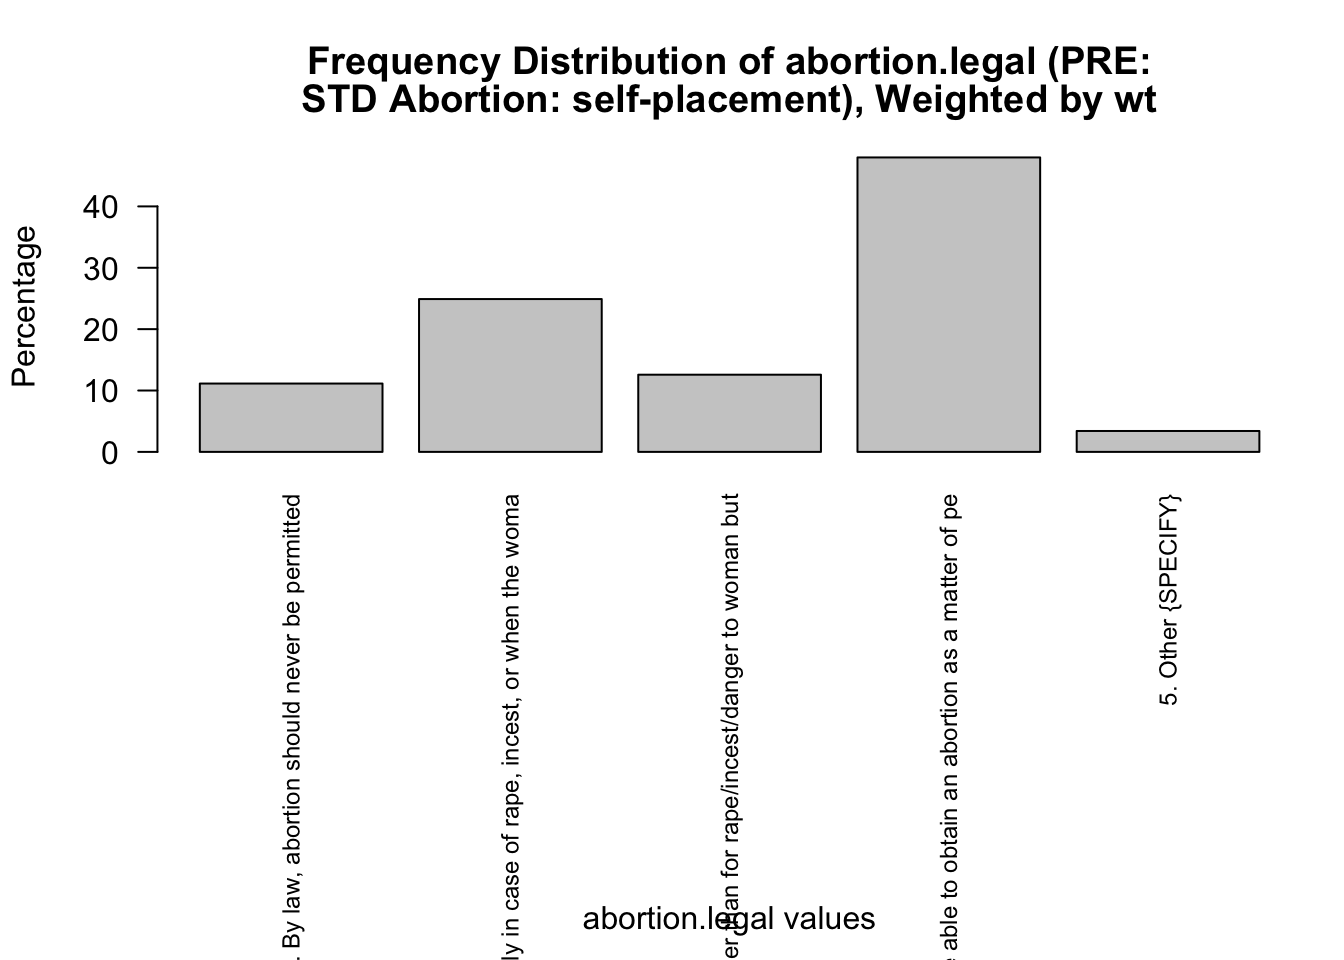
\includegraphics{psc-253-manual_files/figure-latex/unnamed-chunk-72-1.pdf}

\hypertarget{troubleshooting-26}{%
\subsection{Troubleshooting}\label{troubleshooting-26}}

\begin{itemize}
\tightlist
\item
  Alternatively, you can ignore the \texttt{data} argument and specify \texttt{x} and \texttt{w} using the \texttt{data\$variable} notation.
\item
  Remember to use the weights for survey data. The frequency table will be incorrect otherwise.
\item
  There is also a function called \texttt{freq()} that uses different arguments. It is easy to inadvertently use that function. Make sure that you are using \texttt{freqC()}.
\item
  This function requires the \texttt{RCPA3} package.
\end{itemize}

\hypertarget{mode}{%
\section{Calculate the Mode}\label{mode}}

The mode tells us the value of the variable that has the largest number of observations. We could glean this information from a frequency table, but it is more straightforward to have R calculate the mode directly.

\hypertarget{problem-31}{%
\subsection{Problem}\label{problem-31}}

You want to calculate the mode of a variable.

\hypertarget{solution-30}{%
\subsection{Solution}\label{solution-30}}

\begin{enumerate}
\def\labelenumi{\arabic{enumi}.}
\tightlist
\item
  Use the function \texttt{wtd.mode()}.
\item
  Set the \texttt{data} argument to the name of your dataset.
\item
  Set the argument \texttt{x} to the name of the variable for which a mode is being calculated.
\item
  If you have survey data, then set the \texttt{w} argument to the name of the weights variable.
\end{enumerate}

\begin{Shaded}
\begin{Highlighting}[]
\CommentTok{\# Use \textasciigrave{}wtd.mode()\textasciigrave{}}
\FunctionTok{wtd.mode}\NormalTok{(}
  
  \CommentTok{\# set data to the name of the dataset}
  \AttributeTok{data =}\NormalTok{ dataset,}
  
  \CommentTok{\# set x to the name of the variable}
  \AttributeTok{x =}\NormalTok{ variable\_name,}
  
  \CommentTok{\# set w to the weights (only for survey data)}
  \AttributeTok{w =}\NormalTok{ weights\_name}
\NormalTok{)}
\end{Highlighting}
\end{Shaded}

In the example below, we calculate the mode of \texttt{abortion.legal} in the \texttt{nes} dataset. The name of the weight is \texttt{wt}.

\begin{Shaded}
\begin{Highlighting}[]
\CommentTok{\# Use \textasciigrave{}wtd.mode()\textasciigrave{}}
\FunctionTok{wtd.mode}\NormalTok{(}
  
  \CommentTok{\# set data to the name of the dataset}
  \AttributeTok{data =}\NormalTok{ nes,}
  
  \CommentTok{\# set x to the name of the variable}
  \AttributeTok{x =}\NormalTok{ abortion.legal,}
  
  \CommentTok{\# set w to the weights (only for survey data)}
  \AttributeTok{w =}\NormalTok{ wt}
\NormalTok{)}
\end{Highlighting}
\end{Shaded}

\begin{verbatim}
## [1] "4. By law, a woman should always be able to obtain an abortion as a matter of pe"
\end{verbatim}

\hypertarget{troubleshooting-27}{%
\subsection{Troubleshooting}\label{troubleshooting-27}}

\begin{itemize}
\tightlist
\item
  Alternatively, you can ignore the \texttt{data} argument and specify \texttt{x} and \texttt{w} using the \texttt{data\$variable} notation.
\item
  Remember to use the weights for survey data. The mode could be incorrect otherwise.
\item
  This function requires the \texttt{RCPA3} package.
\end{itemize}

\hypertarget{median}{%
\section{Calculate the Median}\label{median}}

The median tells us the value of the variable that splits the data in half.

\hypertarget{problem-32}{%
\subsection{Problem}\label{problem-32}}

You want to calculate the median of a variable.

\hypertarget{solution-31}{%
\subsection{Solution}\label{solution-31}}

\begin{enumerate}
\def\labelenumi{\arabic{enumi}.}
\tightlist
\item
  Use the function \texttt{wtd.median()}.
\item
  Set the \texttt{data} argument to the name of your dataset.
\item
  Set the argument \texttt{x} to the name of the variable for which a mode is being calculated.
\item
  If you have survey data, then set the \texttt{w} argument to the name of the weights variable.
\end{enumerate}

\begin{Shaded}
\begin{Highlighting}[]
\CommentTok{\# Use \textasciigrave{}wtd.median()\textasciigrave{}}
\FunctionTok{wtd.median}\NormalTok{(}
  
  \CommentTok{\# set data to the name of the dataset}
  \AttributeTok{data =}\NormalTok{ dataset,}
  
  \CommentTok{\# set x to the name of the variable}
  \AttributeTok{x =}\NormalTok{ variable\_name,}
  
  \CommentTok{\# set w to the weights (only for survey data)}
  \AttributeTok{w =}\NormalTok{ weights\_name}
\NormalTok{)}
\end{Highlighting}
\end{Shaded}

In the example below, we calculate the median of \texttt{abortion.legal} in the \texttt{nes} dataset. The name of the weight is \texttt{wt}.

\begin{Shaded}
\begin{Highlighting}[]
\CommentTok{\# Use \textasciigrave{}wtd.median()\textasciigrave{}}
\FunctionTok{wtd.median}\NormalTok{(}
  
  \CommentTok{\# set data to the name of the dataset}
  \AttributeTok{data =}\NormalTok{ nes,}
  
  \CommentTok{\# set x to the name of the variable}
  \AttributeTok{x =}\NormalTok{ abortion.legal,}
  
  \CommentTok{\# set w to the weights (only for survey data)}
  \AttributeTok{w =}\NormalTok{ wt}
\NormalTok{)}
\end{Highlighting}
\end{Shaded}

\begin{verbatim}
## [1] "4. By law, a woman should always be able to obtain an abortion as a matter of pe"
\end{verbatim}

\hypertarget{troubleshooting-28}{%
\subsection{Troubleshooting}\label{troubleshooting-28}}

\begin{itemize}
\tightlist
\item
  Alternatively, you can ignore the \texttt{data} argument and specify \texttt{x} and \texttt{w} using the \texttt{data\$variable} notation.
\item
  Remember to use the weights for survey data. The mode could be incorrect otherwise.
\item
  You can only calculate the median if the variable is ordinal or interval.
\item
  This function requires the \texttt{RCPA3} package.
\end{itemize}

\hypertarget{mean}{%
\section{Calculate the Mean}\label{mean}}

The mean is total sum of values of a variable divided by the number of observations. This is what we typically think of when we use the term `average'.

\hypertarget{problem-33}{%
\subsection{Problem}\label{problem-33}}

You want to calculate the mean of a variable.

\hypertarget{solution-32}{%
\subsection{Solution}\label{solution-32}}

\begin{enumerate}
\def\labelenumi{\arabic{enumi}.}
\tightlist
\item
  Use the function \texttt{wtd.mean()}.
\item
  Set the \texttt{data} argument to the name of your dataset.
\item
  Set the argument \texttt{x} to the name of the variable for which a mode is being calculated.
\item
  If you have survey data, then set the \texttt{w} argument to the name of the weights variable.
\end{enumerate}

\begin{Shaded}
\begin{Highlighting}[]
\CommentTok{\# Use \textasciigrave{}wtd.mean()\textasciigrave{}}
\FunctionTok{wtd.mean}\NormalTok{(}
  
  \CommentTok{\# set data to the name of the dataset}
  \AttributeTok{data =}\NormalTok{ dataset,}
  
  \CommentTok{\# set x to the name of the variable}
  \AttributeTok{x =}\NormalTok{ variable\_name,}
  
  \CommentTok{\# set w to the weights (only for survey data)}
  \AttributeTok{w =}\NormalTok{ weights\_name}
\NormalTok{)}
\end{Highlighting}
\end{Shaded}

In the example below, we calculate the mean of \texttt{ft.biden.post} in the \texttt{nes} dataset. The name of the weight is \texttt{wt}.

\begin{Shaded}
\begin{Highlighting}[]
\CommentTok{\# Use \textasciigrave{}wtd.mean()\textasciigrave{}}
\FunctionTok{wtd.mean}\NormalTok{(}
  
  \CommentTok{\# set data to the name of the dataset}
  \AttributeTok{data =}\NormalTok{ nes,}
  
  \CommentTok{\# set x to the name of the variable}
  \AttributeTok{x =}\NormalTok{ ft.biden.post,}
  
  \CommentTok{\# set w to the weights (only for survey data)}
  \AttributeTok{w =}\NormalTok{ wt}
\NormalTok{)}
\end{Highlighting}
\end{Shaded}

\begin{verbatim}
## [1] 52.307
\end{verbatim}

\hypertarget{troubleshooting-29}{%
\subsection{Troubleshooting}\label{troubleshooting-29}}

\begin{itemize}
\tightlist
\item
  Alternatively, you can ignore the \texttt{data} argument and specify \texttt{x} and \texttt{w} using the \texttt{data\$variable} notation.
\item
  Remember to use the weights for survey data. The mode could be incorrect otherwise.
\item
  You can only calculate the mean if the variable is interval.
\item
  This function requires the \texttt{RCPA3} package.
\end{itemize}

\hypertarget{describe}{%
\section{Describe a Variable}\label{describe}}

\hypertarget{problem-34}{%
\subsection{Problem}\label{problem-34}}

You want a general description of a variable.

\hypertarget{solution-33}{%
\subsection{Solution}\label{solution-33}}

\begin{enumerate}
\def\labelenumi{\arabic{enumi}.}
\tightlist
\item
  Use the function \texttt{describeC()}.
\item
  Set the \texttt{data} argument to the name of your dataset.
\item
  Set the argument \texttt{x} to the name of the variable for which a mode is being calculated.
\item
  If you have survey data, then set the \texttt{w} argument to the name of the weights variable.
\end{enumerate}

\begin{Shaded}
\begin{Highlighting}[]
\CommentTok{\# Use \textasciigrave{}describeC()\textasciigrave{}}
\FunctionTok{describeC}\NormalTok{(}
  
  \CommentTok{\# set data to the name of the dataset}
  \AttributeTok{data =}\NormalTok{ dataset,}
  
  \CommentTok{\# set x to the name of the variable}
  \AttributeTok{x =}\NormalTok{ variable\_name,}
  
  \CommentTok{\# set w to the weights (only for survey data)}
  \AttributeTok{w =}\NormalTok{ weights\_name}
\NormalTok{)}
\end{Highlighting}
\end{Shaded}

In the example below, we provide a description of \texttt{ft.biden.post} in the \texttt{nes} dataset. The name of the weight is \texttt{wt}.

\begin{Shaded}
\begin{Highlighting}[]
\CommentTok{\# Use \textasciigrave{}describeC()\textasciigrave{}}
\FunctionTok{describeC}\NormalTok{(}
  
  \CommentTok{\# set data to the name of the dataset}
  \AttributeTok{data =}\NormalTok{ nes,}
  
  \CommentTok{\# set x to the name of the variable}
  \AttributeTok{x =}\NormalTok{ ft.biden.post,}
  
  \CommentTok{\# set w to the weights (only for survey data)}
  \AttributeTok{w =}\NormalTok{ wt}
\NormalTok{)}
\end{Highlighting}
\end{Shaded}

\begin{verbatim}
## ===========================================================================
##                           Descriptive Statistics
## ===========================================================================
## 
## 
## Table: \label{tab:unnamed-chunk-80}Descriptive Statistics for ft.biden.post, weighted by wt
## 
##                              ft.biden.post
## --------------------------  --------------
## Observed values                   7256.644
## Missing values                    1023.356
## Unique values                           64
## Class                              numeric
## Mean                                52.307
## Median                                  60
## Mode                                     0
## Variance                           1268.51
## Standard deviation                  35.616
## Minimum                                  0
## Maximum                                100
## Range                                  100
## First quartile (25%)                    15
## Third quartile (75%)                    85
## Interquartile range (IQR)               70
## Skewness                            -0.222
## Kurtosis                             1.553
\end{verbatim}

\hypertarget{troubleshooting-30}{%
\subsection{Troubleshooting}\label{troubleshooting-30}}

\begin{itemize}
\tightlist
\item
  The function works with all levels of measurement, but it is most useful for interval variables.
\item
  Alternatively, you can ignore the \texttt{data} argument and specify \texttt{x} and \texttt{w} using the \texttt{data\$variable} notation.
\item
  Remember to use the weights for survey data. The mode could be incorrect otherwise.
\item
  This function requires the \texttt{RCPA3} package.
\end{itemize}

\hypertarget{range}{%
\section{Calculate the Range}\label{range}}

The range of a variable tells you the lowest and highest value. This can only be calculated for interval variables.

\hypertarget{problem-35}{%
\subsection{Problem}\label{problem-35}}

You want to calculate the range of an interval variable.

\hypertarget{solution-34}{%
\subsection{Solution}\label{solution-34}}

\begin{enumerate}
\def\labelenumi{\arabic{enumi}.}
\tightlist
\item
  Use the \texttt{range()} function.
\item
  The argument is the name of the variable that you want the range of using the format \texttt{data\$variable}.
\item
  Set the argument \texttt{na.rm} equal to True.
\end{enumerate}

\begin{Shaded}
\begin{Highlighting}[]
\CommentTok{\# Use the range() function}
\FunctionTok{range}\NormalTok{(}
  
  \CommentTok{\# enter the name of the dataset and the name of the variable}
\NormalTok{  dataset}\SpecialCharTok{$}\NormalTok{variable\_name,}
  
  \CommentTok{\# set na.rm=T}
  \AttributeTok{na.rm =}\NormalTok{ T}
\NormalTok{)}
\end{Highlighting}
\end{Shaded}

In the example below, we find the range of the variable \texttt{ft.biden.post}. The dataset is called \texttt{nes}.

\begin{Shaded}
\begin{Highlighting}[]
\CommentTok{\# Use the range() function}
\FunctionTok{range}\NormalTok{(}
  
  \CommentTok{\# enter the name of the dataset and the name of the variable}
\NormalTok{  nes}\SpecialCharTok{$}\NormalTok{ft.biden.post,}
  
  \CommentTok{\# set na.rm=T}
  \AttributeTok{na.rm =}\NormalTok{ T}
\NormalTok{)}
\end{Highlighting}
\end{Shaded}

\begin{verbatim}
## [1]   0 100
\end{verbatim}

\hypertarget{troubleshooting-31}{%
\subsection{Troubleshooting}\label{troubleshooting-31}}

\begin{itemize}
\tightlist
\item
  No common mistakes identified.
\end{itemize}

\hypertarget{barchart_nosurv}{%
\section{Make a Bar Chart of One Variable for non-Survey Data}\label{barchart_nosurv}}

We can use a bar chart to visualize the dispersion for nominal or ordinal variables.

\hypertarget{problem-36}{%
\subsection{Problem}\label{problem-36}}

You want to make a bar chart to visualize the dispersion of one variable when we do not have survey data.

\hypertarget{solution-35}{%
\subsection{Solution}\label{solution-35}}

\begin{enumerate}
\def\labelenumi{\arabic{enumi}.}
\tightlist
\item
  Create a plot object. I typically name my plots something simple like \texttt{p1}.
\item
  Assign the function \texttt{ggplot()} to the plot object.
\item
  Set the argument \texttt{data} to the name of your dataset.
\item
  Set the argument \texttt{mapping} to the function \texttt{aes()}.

  \begin{enumerate}
  \def\labelenumii{\alph{enumii}.}
  \tightlist
  \item
    Inside the \texttt{aes()} function, set the argument \texttt{x} to the name of your variable.
  \item
    Set the argument \texttt{fill} to the name of your variable.
  \end{enumerate}
\item
  Make sure all the parentheses are closed and type a \texttt{+} sign.
\item
  Use the function \texttt{geom\_bar()} to draw the bar. The function will not have any arguments.
\item
  Call the plot object by typing its name.
\end{enumerate}

\begin{Shaded}
\begin{Highlighting}[]
\CommentTok{\# assign ggplot() to a new plot object}
\NormalTok{p1 }\OtherTok{\textless{}{-}} \FunctionTok{ggplot}\NormalTok{(}
  
  \CommentTok{\# set data to the name of the dataset}
  \AttributeTok{data =}\NormalTok{ dataset,}
  
  \CommentTok{\# set \textasciigrave{}mapping\textasciigrave{} to the function \textasciigrave{}aes()\textasciigrave{}}
  \AttributeTok{mapping =} \FunctionTok{aes}\NormalTok{(}
    
    \CommentTok{\# set \textasciigrave{}x\textasciigrave{} to the name of the variable}
    \AttributeTok{x =}\NormalTok{ variable\_name,}
    
    \CommentTok{\# set \textasciigrave{}fill\textasciigrave{} to the name of the variable}
    \AttributeTok{fill =}\NormalTok{ variable\_name}
\NormalTok{  )}
  
  \CommentTok{\# close parentheses and type a + sign}
\NormalTok{) }\SpecialCharTok{+}
  
  \CommentTok{\# use the function \textasciigrave{}geom\_bar()\textasciigrave{}}
  \FunctionTok{geom\_bar}\NormalTok{()}

\CommentTok{\# call the plot}
\NormalTok{p1}
\end{Highlighting}
\end{Shaded}

In the example below, we create a bar chart for the variable \texttt{gay.policy2}. The name of the dataset is \texttt{states}.

\begin{Shaded}
\begin{Highlighting}[]
\CommentTok{\# assign ggplot() to a new plot object}
\NormalTok{p1 }\OtherTok{\textless{}{-}} \FunctionTok{ggplot}\NormalTok{(}
  
  \CommentTok{\# set data to the name of the dataset}
  \AttributeTok{data =}\NormalTok{ states,}
  
  \CommentTok{\# set \textasciigrave{}mapping\textasciigrave{} to the function \textasciigrave{}aes()\textasciigrave{}}
  \AttributeTok{mapping =} \FunctionTok{aes}\NormalTok{(}
    
    \CommentTok{\# set \textasciigrave{}x\textasciigrave{} to the name of the variable}
    \AttributeTok{x =}\NormalTok{ gay.policy2,}
    
    \CommentTok{\# set \textasciigrave{}fill\textasciigrave{} to the name of the variable}
    \AttributeTok{fill =}\NormalTok{ gay.policy2}
\NormalTok{  )}
  
  \CommentTok{\# close parentheses and type a + sign}
\NormalTok{) }\SpecialCharTok{+}
  
  \CommentTok{\# use the function \textasciigrave{}geom\_bar()\textasciigrave{}}
  \FunctionTok{geom\_bar}\NormalTok{()}

\CommentTok{\# call the plot}
\NormalTok{p1}
\end{Highlighting}
\end{Shaded}

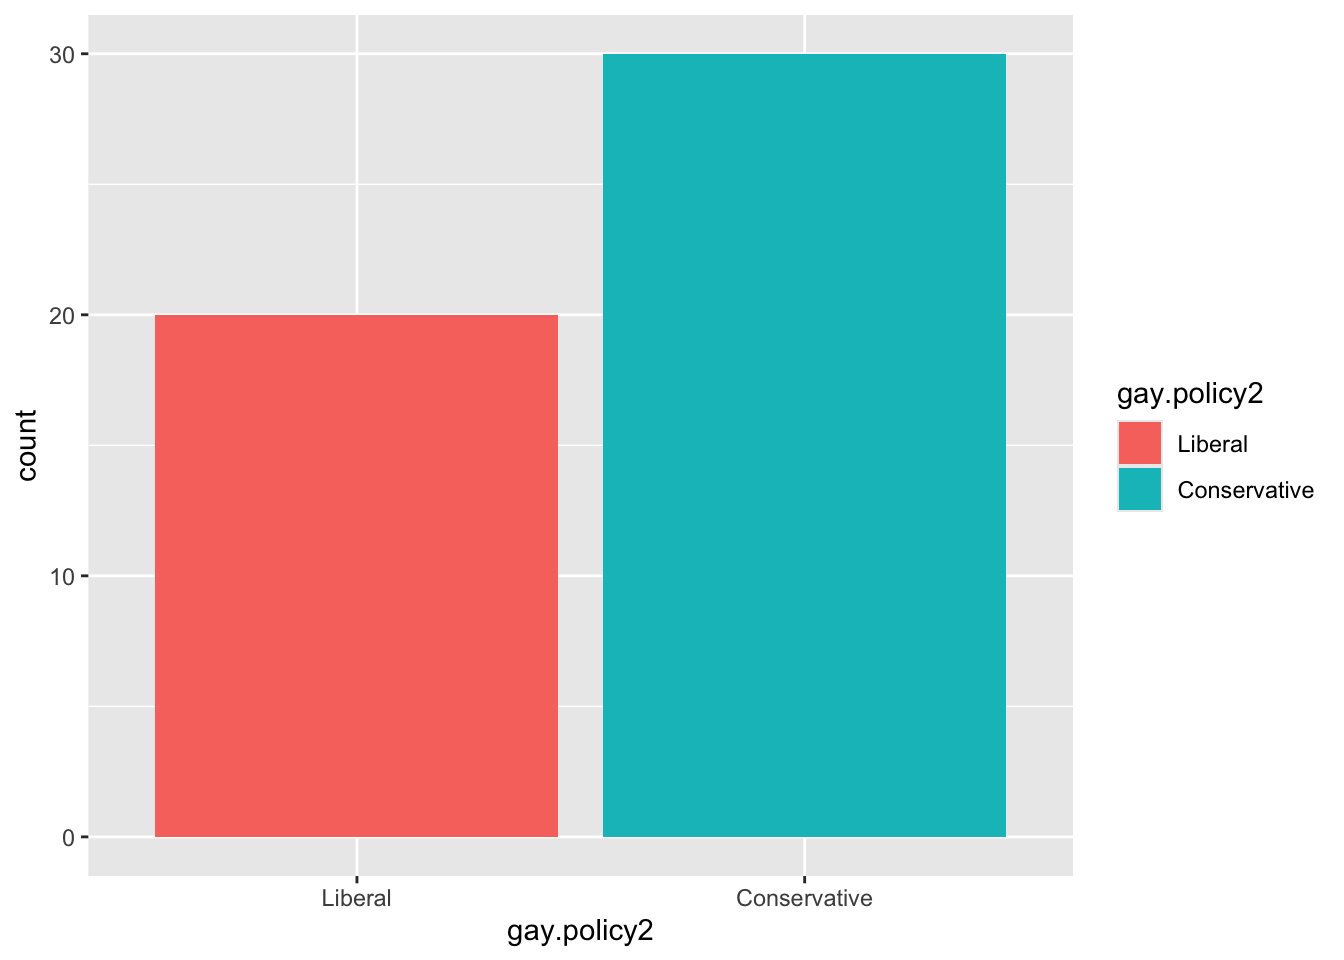
\includegraphics{psc-253-manual_files/figure-latex/unnamed-chunk-84-1.pdf}

\hypertarget{troubleshooting-32}{%
\subsection{Troubleshooting}\label{troubleshooting-32}}

\begin{itemize}
\item
  Make sure that all arguments are separated by a comma, and that you use a \texttt{+} sign to connect the \texttt{ggplot()} function to the \texttt{geom\_bar()} function.
\item
  Remember to call the plot. If you do not type the name of the plot object (\texttt{p1} in the example above), then R will not show what the plot looks like.
\end{itemize}

\hypertarget{histNoSurvey}{%
\section{Make a Histogram (for non survey data)}\label{histNoSurvey}}

We use histograms to visualize the dispersion of an interval variable.

\hypertarget{problem-37}{%
\subsection{Problem}\label{problem-37}}

You want to make a histogram, and you do not have survey data.

\hypertarget{solution-36}{%
\subsection{Solution}\label{solution-36}}

\begin{enumerate}
\def\labelenumi{\arabic{enumi}.}
\tightlist
\item
  Assign the function \texttt{ggplot()} to a new plot object. A simple name like \texttt{p1} is fine.
\item
  Set the argument \texttt{data} to the name of your dataset.
\item
  Set the argument \texttt{mapping} to the function \texttt{aes()}.
\item
  Inside the \texttt{aes()} function, set the argument \texttt{x} to the name of your variable.
\item
  Make sure all the parentheses are closed and type a \texttt{+} sign after the last parenthesis.
\item
  Use the function \texttt{geom\_histogram()} to draw the histogram bars. The function will not have any arguments.
\item
  Call the plot object by typing its name.
\end{enumerate}

\begin{Shaded}
\begin{Highlighting}[]
\CommentTok{\# assign ggplot() to a new plot object}
\NormalTok{p2 }\OtherTok{\textless{}{-}} \FunctionTok{ggplot}\NormalTok{(}
  
  \CommentTok{\# set data to the name of the dataset}
  \AttributeTok{data =}\NormalTok{ dataset,}
  
  \CommentTok{\# set \textasciigrave{}mapping\textasciigrave{} to the function \textasciigrave{}aes()\textasciigrave{}}
  \AttributeTok{mapping =} \FunctionTok{aes}\NormalTok{(}
    
    \CommentTok{\# set \textasciigrave{}x\textasciigrave{} to the name of the variable}
    \AttributeTok{x =}\NormalTok{ variable\_name}
\NormalTok{  )}
  
  \CommentTok{\# close parentheses and type a + sign}
\NormalTok{) }\SpecialCharTok{+}
  
  \CommentTok{\# use the function \textasciigrave{}geom\_histogram()\textasciigrave{}}
  \FunctionTok{geom\_histogram}\NormalTok{()}

\CommentTok{\# call the plot}
\NormalTok{p2}
\end{Highlighting}
\end{Shaded}

In the example below we create a histogram of Biden's share of the vote in 2020, \texttt{biden2020}, which is found in the \texttt{states} dataset.

\begin{Shaded}
\begin{Highlighting}[]
\CommentTok{\# assign ggplot() to a new plot object}
\NormalTok{p2 }\OtherTok{\textless{}{-}} \FunctionTok{ggplot}\NormalTok{(}
  
  \CommentTok{\# set data to the name of the dataset}
  \AttributeTok{data =}\NormalTok{ states,}
  
  \CommentTok{\# set \textasciigrave{}mapping\textasciigrave{} to the function \textasciigrave{}aes()\textasciigrave{}}
  \AttributeTok{mapping =} \FunctionTok{aes}\NormalTok{(}
    
    \CommentTok{\# set \textasciigrave{}x\textasciigrave{} to the name of the variable}
    \AttributeTok{x =}\NormalTok{ biden2020}
\NormalTok{  )}
  
  \CommentTok{\# close parentheses and type a + sign}
\NormalTok{) }\SpecialCharTok{+}
  
  \CommentTok{\# use the function \textasciigrave{}geom\_histogram()\textasciigrave{}}
  \FunctionTok{geom\_histogram}\NormalTok{()}

\CommentTok{\# call the plot}
\NormalTok{p2}
\end{Highlighting}
\end{Shaded}

\begin{verbatim}
## `stat_bin()` using `bins = 30`. Pick better value with `binwidth`.
\end{verbatim}

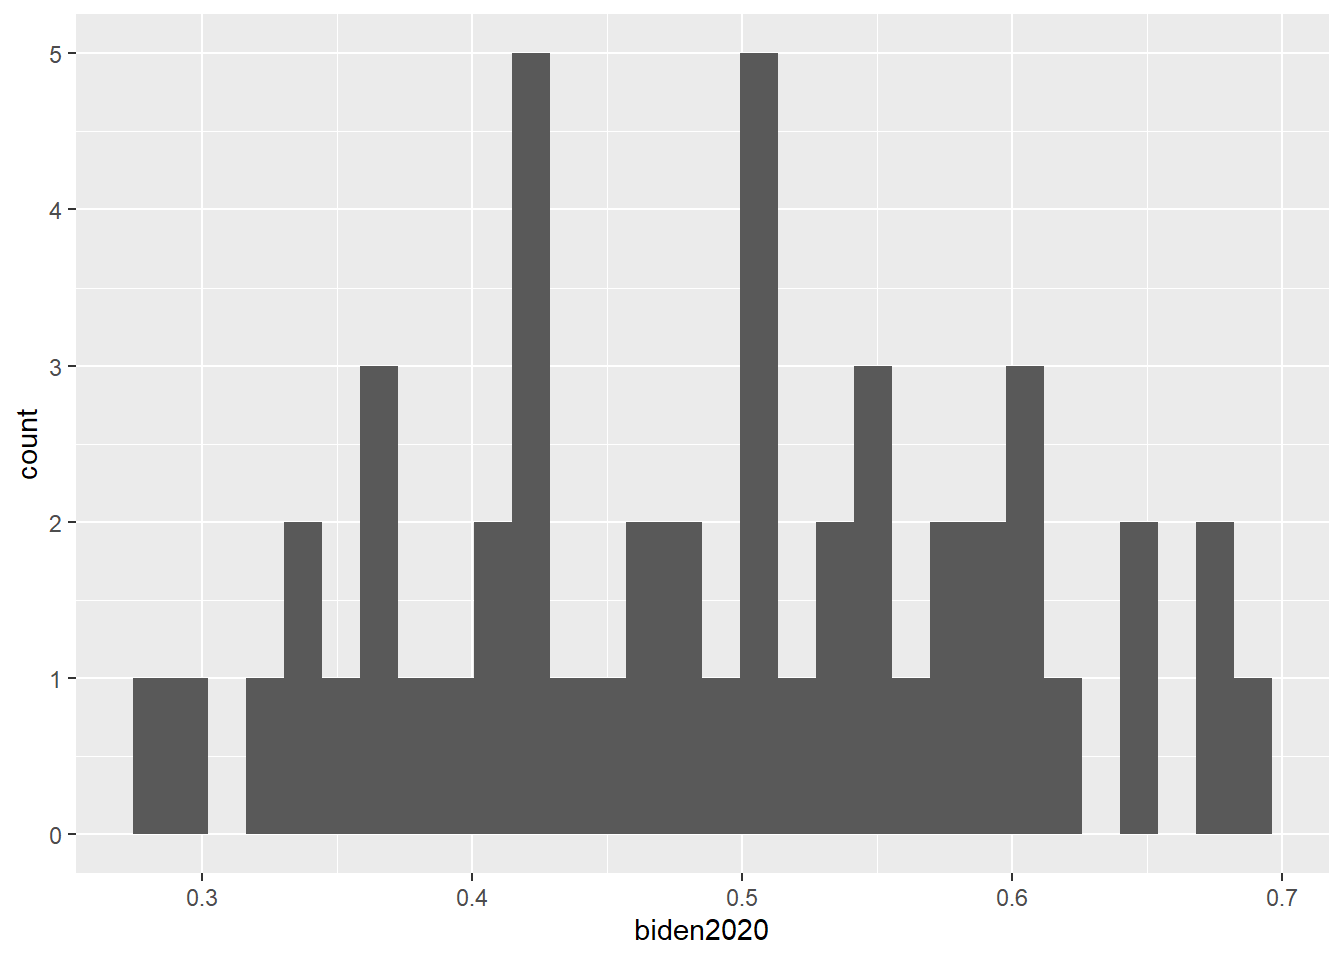
\includegraphics{psc-253-manual_files/figure-latex/unnamed-chunk-86-1.pdf}

\hypertarget{troubleshooting-33}{%
\subsection{Troubleshooting}\label{troubleshooting-33}}

\begin{itemize}
\item
  Make sure that all arguments are separated by a comma, and that you use a \texttt{+} sign to connect the \texttt{ggplot()} function to the \texttt{geom\_histogram()} function.
\item
  Remember to call the plot. If you do not type the name of the plot object (\texttt{p1} in the example above), then R will not show what the plot looks like.
\item
  You can use the argument \texttt{binwidth} inside \texttt{geom\_histogram()} to control the size and number of bars that are drawn.
\end{itemize}

\hypertarget{histSurvey}{%
\section{Make a Histogram (for survey data)}\label{histSurvey}}

We use histograms to visualize the dispersion of an interval variable.

\hypertarget{problem-38}{%
\subsection{Problem}\label{problem-38}}

You want to make a histogram, and you do have survey data.

\hypertarget{solution-37}{%
\subsection{Solution}\label{solution-37}}

\begin{enumerate}
\def\labelenumi{\arabic{enumi}.}
\tightlist
\item
  Use the function \texttt{histC()}.
\item
  Set the \texttt{data} argument to the name of your dataset.
\item
  Set the argument \texttt{x} to the name of the variable for which a mode is being calculated.
\item
  If you have survey data, then set the \texttt{w} argument to the name of the weights variable.
\end{enumerate}

\begin{Shaded}
\begin{Highlighting}[]
\CommentTok{\# Use \textasciigrave{}histC()\textasciigrave{}}
\FunctionTok{histC}\NormalTok{(}
  
  \CommentTok{\# set data to the name of the dataset}
  \AttributeTok{data =}\NormalTok{ dataset,}
  
  \CommentTok{\# set x to the name of the variable}
  \AttributeTok{x =}\NormalTok{ variable\_name,}
  
  \CommentTok{\# set w to the weights (only for survey data)}
  \AttributeTok{w =}\NormalTok{ weights\_name}
\NormalTok{)}
\end{Highlighting}
\end{Shaded}

In the example below we create a histogram of the feeling thermometer for Biden, \texttt{ft.biden.post}, which is found in the \texttt{nes} dataset.

\begin{Shaded}
\begin{Highlighting}[]
\CommentTok{\# Use \textasciigrave{}histC()\textasciigrave{}}
\FunctionTok{histC}\NormalTok{(}
  
  \CommentTok{\# set data to the name of the dataset}
  \AttributeTok{data =}\NormalTok{ nes,}
  
  \CommentTok{\# set x to the name of the variable}
  \AttributeTok{x =}\NormalTok{ ft.biden.post,}
  
  \CommentTok{\# set w to the weights (only for survey data)}
  \AttributeTok{w =}\NormalTok{ wt}
\NormalTok{)}
\end{Highlighting}
\end{Shaded}

\begin{verbatim}
## ===========================================================================
##    Describing Distribution of Values with Frequency Table and Histogram
## ===========================================================================
## 
## 
## Table: \label{tab:unnamed-chunk-88}Distribution of Binned Values of ft.biden.post, Weighted by wt
## 
##    Interval   Frequency   Percent   Cum. Percent
## -----------  ----------  --------  -------------
##    [0 - 10]     1488.88     20.52          20.52
##   (10 - 20]      543.26      7.49          28.01
##   (20 - 30]      456.12      6.29          34.30
##   (30 - 40]      395.48      5.45          39.75
##   (40 - 50]      507.50      6.99          46.74
##   (50 - 60]      588.70      8.11          54.85
##   (60 - 70]      875.94     12.07          66.92
##   (70 - 80]      194.96      2.69          69.61
##   (80 - 90]     1090.03     15.02          84.63
##  (90 - 100]     1115.77     15.38         100.01
##       Total     7256.64    100.00             NA
\end{verbatim}

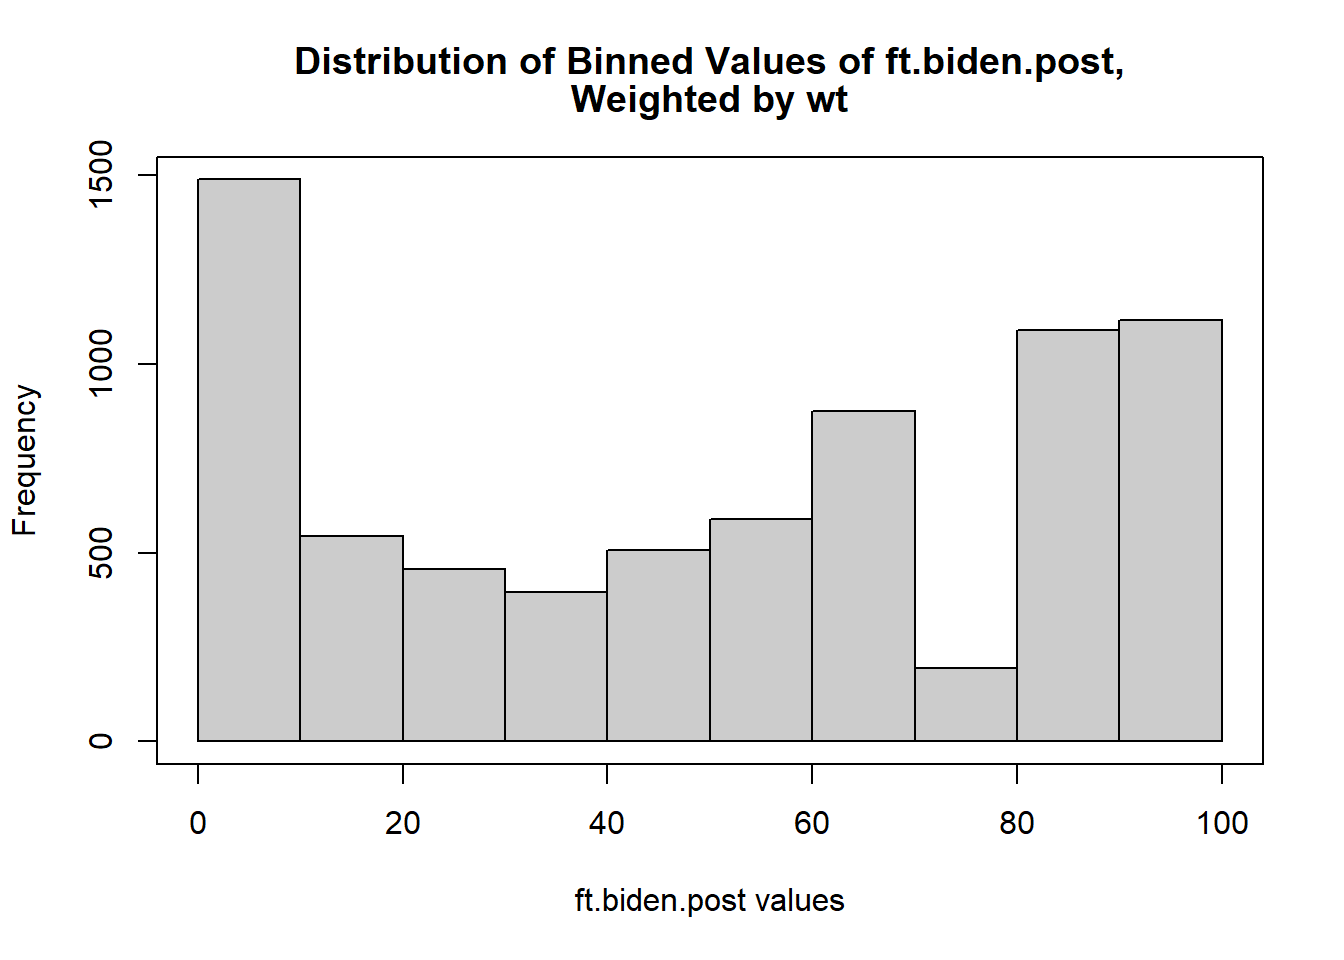
\includegraphics{psc-253-manual_files/figure-latex/unnamed-chunk-88-1.pdf}

\hypertarget{troubleshooting-34}{%
\subsection{Troubleshooting}\label{troubleshooting-34}}

\begin{itemize}
\item
  Alternatively, you can ignore the \texttt{data} argument and specify \texttt{x} and \texttt{w} using the \texttt{data\$variable} notation.
\item
  Remember to use the weights for survey data.
\item
  This function requires the \texttt{RCPA3} package.
\end{itemize}

\hypertarget{boxplot}{%
\section{Make a Boxplot}\label{boxplot}}

We can use a boxplot as an alternative way to visualize the dispersion of an interval variable.

\hypertarget{problem-39}{%
\subsection{Problem}\label{problem-39}}

You want to make a boxplot.

\hypertarget{solution-38}{%
\subsection{Solution}\label{solution-38}}

\begin{enumerate}
\def\labelenumi{\arabic{enumi}.}
\tightlist
\item
  Assign the function \texttt{ggplot()} to a new plot object. A simple name like \texttt{p1} is fine.
\item
  Set the argument \texttt{data} to the name of your dataset.
\item
  Set the argument \texttt{mapping} to the function \texttt{aes()}.
\item
  Inside the \texttt{aes()} function, set the argument \texttt{y} to the name of your variable.
\item
  Make sure all the parentheses are closed and type a \texttt{+} sign after the last parenthesis.
\item
  Use the function \texttt{geom\_boxplot()} to draw the box shape. The function will not have any arguments.
\item
  Call the plot object by typing its name.
\end{enumerate}

\begin{Shaded}
\begin{Highlighting}[]
\CommentTok{\# assign ggplot() to a new plot object}
\NormalTok{p3 }\OtherTok{\textless{}{-}} \FunctionTok{ggplot}\NormalTok{(}
  
  \CommentTok{\# set data to the name of the dataset}
  \AttributeTok{data =}\NormalTok{ dataset,}
  
  \CommentTok{\# set \textasciigrave{}mapping\textasciigrave{} to the function \textasciigrave{}aes()\textasciigrave{}}
  \AttributeTok{mapping =} \FunctionTok{aes}\NormalTok{(}
    
    \CommentTok{\# set \textasciigrave{}x\textasciigrave{} to the name of the variable}
    \AttributeTok{x =}\NormalTok{ variable\_name}
\NormalTok{  )}
  
  \CommentTok{\# close parentheses and type a + sign}
\NormalTok{) }\SpecialCharTok{+}
  
  \CommentTok{\# use the function \textasciigrave{}geom\_boxplot()\textasciigrave{}}
  \FunctionTok{geom\_boxplot}\NormalTok{()}

\CommentTok{\# call the plot}
\NormalTok{p3}
\end{Highlighting}
\end{Shaded}

In the example below we create a boxplot of Biden's share of the vote in 2020, \texttt{biden2020}, which is found in the \texttt{states} dataset.

\begin{Shaded}
\begin{Highlighting}[]
\CommentTok{\# assign ggplot() to a new plot object}
\NormalTok{p3 }\OtherTok{\textless{}{-}} \FunctionTok{ggplot}\NormalTok{(}
  
  \CommentTok{\# set data to the name of the dataset}
  \AttributeTok{data =}\NormalTok{ states,}
  
  \CommentTok{\# set \textasciigrave{}mapping\textasciigrave{} to the function \textasciigrave{}aes()\textasciigrave{}}
  \AttributeTok{mapping =} \FunctionTok{aes}\NormalTok{(}
    
    \CommentTok{\# set \textasciigrave{}x\textasciigrave{} to the name of the variable}
    \AttributeTok{x =}\NormalTok{ biden2020}
\NormalTok{  )}
  
  \CommentTok{\# close parentheses and type a + sign}
\NormalTok{) }\SpecialCharTok{+}
  
  \CommentTok{\# use the function \textasciigrave{}geom\_boxplot()\textasciigrave{}}
  \FunctionTok{geom\_boxplot}\NormalTok{()}

\CommentTok{\# call the plot}
\NormalTok{p3}
\end{Highlighting}
\end{Shaded}

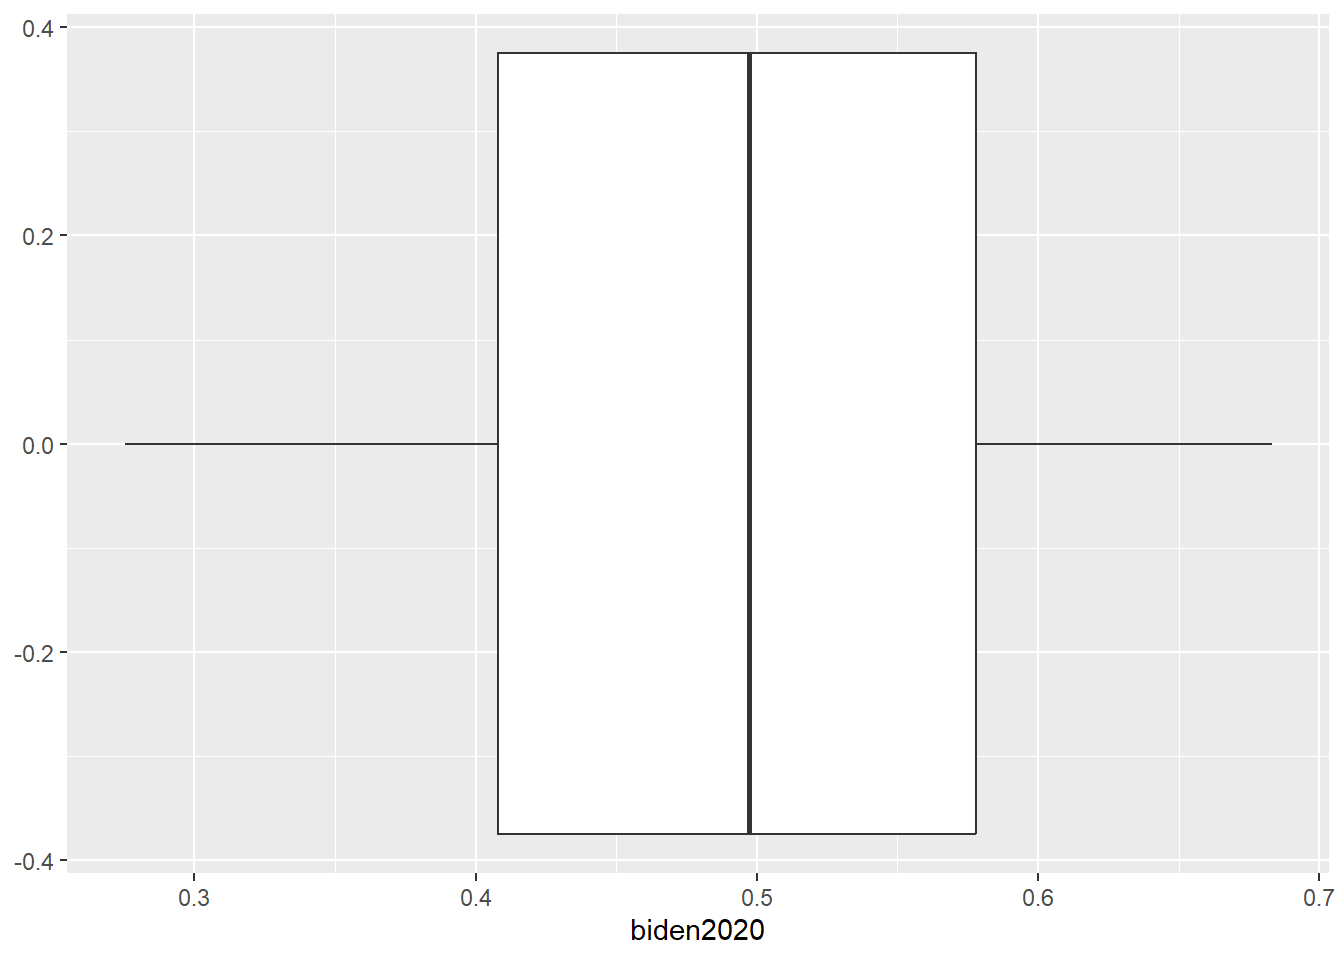
\includegraphics{psc-253-manual_files/figure-latex/unnamed-chunk-90-1.pdf}

\hypertarget{troubleshooting-35}{%
\subsection{Troubleshooting}\label{troubleshooting-35}}

\begin{itemize}
\item
  Make sure that all arguments are separated by a comma, and that you use a \texttt{+} sign to connect the \texttt{ggplot()} function to the \texttt{geom\_boxplot()} function.
\item
  Remember to call the plot. If you do not type the name of the plot object (\texttt{p3} in the example above), then R will not show what the plot looks like.
\end{itemize}

\hypertarget{simple-comparisons}{%
\chapter{Simple Comparisons}\label{simple-comparisons}}

\hypertarget{crosstab}{%
\section{Crosstab}\label{crosstab}}

\hypertarget{problem-40}{%
\subsection{Problem}\label{problem-40}}

You want to make a crosstab.

\hypertarget{solution-39}{%
\subsection{Solution}\label{solution-39}}

\begin{enumerate}
\def\labelenumi{\arabic{enumi}.}
\tightlist
\item
  Load the \texttt{RCPA3} package.
\item
  In order to create a crosstab in R, we use the function called \texttt{crosstabC()}.\\
\item
  The function follows the following template:
\end{enumerate}

\begin{Shaded}
\begin{Highlighting}[]
\CommentTok{\# use the function \textasciigrave{}crosstabC()}
\FunctionTok{crosstabC}\NormalTok{(}
  
  \CommentTok{\# set \textasciigrave{}data\textasciigrave{} equal to your dataset}
  \AttributeTok{data =}\NormalTok{ dataset,}
  
  \CommentTok{\# \textasciigrave{}dv\textasciigrave{} equal to the name of your dependent variable}
  \AttributeTok{dv =}\NormalTok{ dependent\_variable, }
  
  \CommentTok{\# set \textasciigrave{}iv\textasciigrave{} equal to the name of your independent variable}
  \AttributeTok{iv =}\NormalTok{ independent\_variable, }
  
  \CommentTok{\# if you have survey data, set \textasciigrave{}w\textasciigrave{} equal to the name of your weights variable}
  \AttributeTok{w =}\NormalTok{ weights)}
\end{Highlighting}
\end{Shaded}

\begin{enumerate}
\def\labelenumi{\arabic{enumi}.}
\setcounter{enumi}{3}
\tightlist
\item
  Specify the dataset, the dependent variable, the independent variable, and the weights (if applicable)
\end{enumerate}

In this example, we are making a crosstab where the dataset is `nes', the dependent variable is \texttt{abortion.imp}, the independent variable is \texttt{partyid3}, and the weights are called \texttt{wt}.

\begin{Shaded}
\begin{Highlighting}[]
\CommentTok{\# use the function \textasciigrave{}crosstabC()}
\FunctionTok{crosstabC}\NormalTok{(}
  
  \CommentTok{\# set \textasciigrave{}data\textasciigrave{} equal to your dataset}
  \AttributeTok{data =}\NormalTok{ nes,}
  
  \CommentTok{\# \textasciigrave{}dv\textasciigrave{} equal to the name of your dependent variable}
  \AttributeTok{dv =}\NormalTok{ abortion.imp, }
  
  \CommentTok{\# set \textasciigrave{}iv\textasciigrave{} equal to the name of your independent variable}
  \AttributeTok{iv =}\NormalTok{ partyid3, }
  
  \CommentTok{\# if you have survey data, set \textasciigrave{}w\textasciigrave{} equal to the name of your weights variable}
  \AttributeTok{w =}\NormalTok{ wt,}
  \CommentTok{\# do not make the plot}
  \AttributeTok{plot =}\NormalTok{ F)}
\end{Highlighting}
\end{Shaded}

\begin{verbatim}
## ===========================================================================
##                          Cross-Tabulation Analysis
## ===========================================================================
## 
## 
## Table: \label{tab:unnamed-chunk-93}Cross-Tabulation of abortion.imp and partyid3, weighted by wt
## 
##                              1. Democrat   2. Independent   3. Republican    Totals
## --------------------------  ------------  ---------------  --------------  --------
## % 1. Not at all important           3.59             6.82            3.67      4.70
## __Count___                        102.67           188.80           95.39    386.86
## % 2. Not too important             10.31            15.16           14.41     13.23
## __Count___                        294.64           419.74          374.26   1088.64
## % 3. Somewhat important            27.28            29.30           25.65     27.44
## __Count___                        779.82           811.47          666.30   2257.59
## % 4. Very important                29.00            25.49           26.57     27.05
## __Count___                        829.02           705.82          690.36   2225.20
## % 5. Extremely important           29.81            23.24           29.71     27.57
## __Count___                        852.18           643.61          771.78   2267.58
## % Totals                          100.00           100.00          100.00    100.00
## __Count___                       2858.33          2769.44         2598.10   8225.87
\end{verbatim}

\hypertarget{troubleshooting-36}{%
\subsection{Troubleshooting}\label{troubleshooting-36}}

\begin{itemize}
\tightlist
\item
  Make sure that the \texttt{RCPA3} package is loaded. Use \texttt{library(RCPA3)} to load.
\item
  If you specify the data argument, then the arguments for the independent and dependent variables are just the variable names. They do not follow the template of \texttt{data\$variable}.
\item
  If you do not specify the data argument, then the arguments for the independent and dependent variables do follow the template of \texttt{data\$variable}.
\item
  Crosstabs are used when both the independent and dependent variables are categorical. Avoid making a crosstab with numeric data.
\end{itemize}

\hypertarget{compmeans}{%
\section{Comparison of Means}\label{compmeans}}

\hypertarget{problem-41}{%
\subsection{Problem}\label{problem-41}}

You want to make a comparison of means table.

\hypertarget{solution-40}{%
\subsection{Solution}\label{solution-40}}

\begin{enumerate}
\def\labelenumi{\arabic{enumi}.}
\tightlist
\item
  Load the \texttt{RCPA3} package.
\item
  In order to create a comparison of means table in R, we use the function called \texttt{compmeansC()}.\\
\item
  The function follows the following template:
\end{enumerate}

\begin{Shaded}
\begin{Highlighting}[]
\CommentTok{\# use the function \textasciigrave{}compmeansC()}
\FunctionTok{compmeansC}\NormalTok{(}
  
  \CommentTok{\# set \textasciigrave{}data\textasciigrave{} equal to your dataset}
  \AttributeTok{data =}\NormalTok{ dataset,}
  
  \CommentTok{\# \textasciigrave{}dv\textasciigrave{} equal to the name of your dependent variable}
  \AttributeTok{dv =}\NormalTok{ dependent\_variable, }
  
  \CommentTok{\# set \textasciigrave{}iv\textasciigrave{} equal to the name of your independent variable}
  \AttributeTok{iv =}\NormalTok{ independent\_variable, }
  
  \CommentTok{\# if you have survey data, set \textasciigrave{}w\textasciigrave{} equal to the name of your weights variable}
  \AttributeTok{w =}\NormalTok{ weights)}
\end{Highlighting}
\end{Shaded}

Here is a comparison of means table for feelings towards Obama \texttt{ft.obama} by party identification \texttt{partyid3}.

\begin{Shaded}
\begin{Highlighting}[]
\FunctionTok{compmeansC}\NormalTok{(}
  
  \CommentTok{\# set \textasciigrave{}data\textasciigrave{} equal to your dataset}
  \AttributeTok{data =}\NormalTok{ nes,}
  
  \CommentTok{\# \textasciigrave{}dv\textasciigrave{} equal to the name of your dependent variable}
  \AttributeTok{dv =}\NormalTok{ ft.obama, }
  
  \CommentTok{\# set \textasciigrave{}iv\textasciigrave{} equal to the name of your independent variable}
  \AttributeTok{iv =}\NormalTok{ partyid3, }
  
  \CommentTok{\# if you have survey data, set \textasciigrave{}w\textasciigrave{} equal to the name of your weights variable}
  \AttributeTok{w =}\NormalTok{ wt,}
  \CommentTok{\# do not make the plot}
  \AttributeTok{plot =}\NormalTok{ F)}
\end{Highlighting}
\end{Shaded}

\begin{verbatim}
## ===========================================================================
##                          Mean Comparison Analysis
## ===========================================================================
## 
## 
## Table: \label{tab:unnamed-chunk-95}Mean Values of ft.obama by partyid3, Weighted by wt
## 
##                    Mean         N   St. Dev.
## ---------------  ------  --------  ---------
## 1. Democrat       89.90   2839.88      15.45
## 2. Independent    61.67   2748.29      32.33
## 3. Republican     26.98   2578.53      28.30
## Total             60.53   8166.71      36.65
\end{verbatim}

\hypertarget{troubleshooting-37}{%
\subsection{Troubleshooting}\label{troubleshooting-37}}

\begin{itemize}
\tightlist
\item
  Make sure \texttt{RCPA3} is loaded.
\item
  You only need to specify the weights argument if you have survey data with survey weights.
\end{itemize}

\hypertarget{barchart2}{%
\section{Make a Bar Chart for Two Variables}\label{barchart2}}

\hypertarget{problem-42}{%
\subsection{Problem}\label{problem-42}}

Make a barchart that plots the mean of a dependent variable (Y) by an independent variable (X).

\hypertarget{solution-41}{%
\subsection{Solution}\label{solution-41}}

\begin{enumerate}
\def\labelenumi{\arabic{enumi}.}
\tightlist
\item
  \protect\hyperlink{sum}{Create a summary dataset} to plot.
\item
  Use \texttt{ggplot()} for the data and the mapping.
\item
  The data is the summary dataset, \texttt{data\ =\ sum\_data}
\item
  The mapping is \texttt{mapping\ =\ aes(x\ =\ independent,\ y\ =\ dependent)}
\item
  If you want to color the bars, add \texttt{fill\ =\ independent} to the mapping.
\item
  Use a \texttt{+} at the end of the line of code.
\item
  Use \texttt{geom\_col()} to make the bar shapes.
\end{enumerate}

\begin{Shaded}
\begin{Highlighting}[]
\CommentTok{\# create a plot object set to \textasciigrave{}ggplot()\textasciigrave{}}
\NormalTok{p1 }\OtherTok{\textless{}{-}} \FunctionTok{ggplot}\NormalTok{(}
  
  \CommentTok{\# specify the data as the name of your summary data}
  \AttributeTok{data =}\NormalTok{ sum\_data,}
  
  \CommentTok{\# specify the mapping}
  \AttributeTok{mapping =} \FunctionTok{aes}\NormalTok{(}
    
    \CommentTok{\# set x to the name of the independent variable}
    \AttributeTok{x =}\NormalTok{ independent,}
    
    \CommentTok{\# set y to the name of the dependent variable}
    \AttributeTok{y =}\NormalTok{ dependent,}
    
    \CommentTok{\# set \textasciigrave{}fill\textasciigrave{} to the name of the independent variable}
    \AttributeTok{fill =}\NormalTok{ independent)) }\SpecialCharTok{+}
  
  \CommentTok{\# use \textasciigrave{}geom\_col() to create the bars}
  \FunctionTok{geom\_col}\NormalTok{()}

\CommentTok{\# call the plot using the name of your plot object}
\NormalTok{p1}
\end{Highlighting}
\end{Shaded}

Plot the mean feelings towards Obama \texttt{obama\_therm} by party identification \texttt{pid\_x}.

\begin{Shaded}
\begin{Highlighting}[]
\CommentTok{\# create the summary dataset}
\CommentTok{\# assign old data to a new data object}
\NormalTok{partymeans }\OtherTok{\textless{}{-}}\NormalTok{ nes }\SpecialCharTok{\%\textgreater{}\%}
  
  \CommentTok{\# use group\_by() to group the data by partyid7}
  \FunctionTok{group\_by}\NormalTok{(partyid7) }\SpecialCharTok{\%\textgreater{}\%}
  
  \CommentTok{\# calculate the means of ft.obama}
  \FunctionTok{summarise}\NormalTok{(}\AttributeTok{average =} \FunctionTok{wtd.mean}\NormalTok{(ft.obama, }\AttributeTok{na.rm =}\NormalTok{ T,}
                               \AttributeTok{w =}\NormalTok{ wt))}

\CommentTok{\# create a plot object set to \textasciigrave{}ggplot()\textasciigrave{}}
\NormalTok{p1 }\OtherTok{\textless{}{-}} \FunctionTok{ggplot}\NormalTok{(}
  
  \CommentTok{\# specify the data as the name of your summary data}
  \AttributeTok{data =}\NormalTok{ partymeans,}
  
  \CommentTok{\# specify the mapping}
  \AttributeTok{mapping =} \FunctionTok{aes}\NormalTok{(}
    
    \CommentTok{\# set x to the name of the independent variable}
    \AttributeTok{x =}\NormalTok{ partyid7,}
    
    \CommentTok{\# set y to the name of the dependent variable}
    \AttributeTok{y =}\NormalTok{ average,}
    
    \CommentTok{\# set \textasciigrave{}fill\textasciigrave{} to the name of the independent variable}
    \AttributeTok{fill =}\NormalTok{ partyid7)) }\SpecialCharTok{+}
  
  \CommentTok{\# use \textasciigrave{}geom\_col() to create the bars}
  \FunctionTok{geom\_col}\NormalTok{()}

\CommentTok{\# call the plot using the name of your plot object}
\NormalTok{p1}
\end{Highlighting}
\end{Shaded}

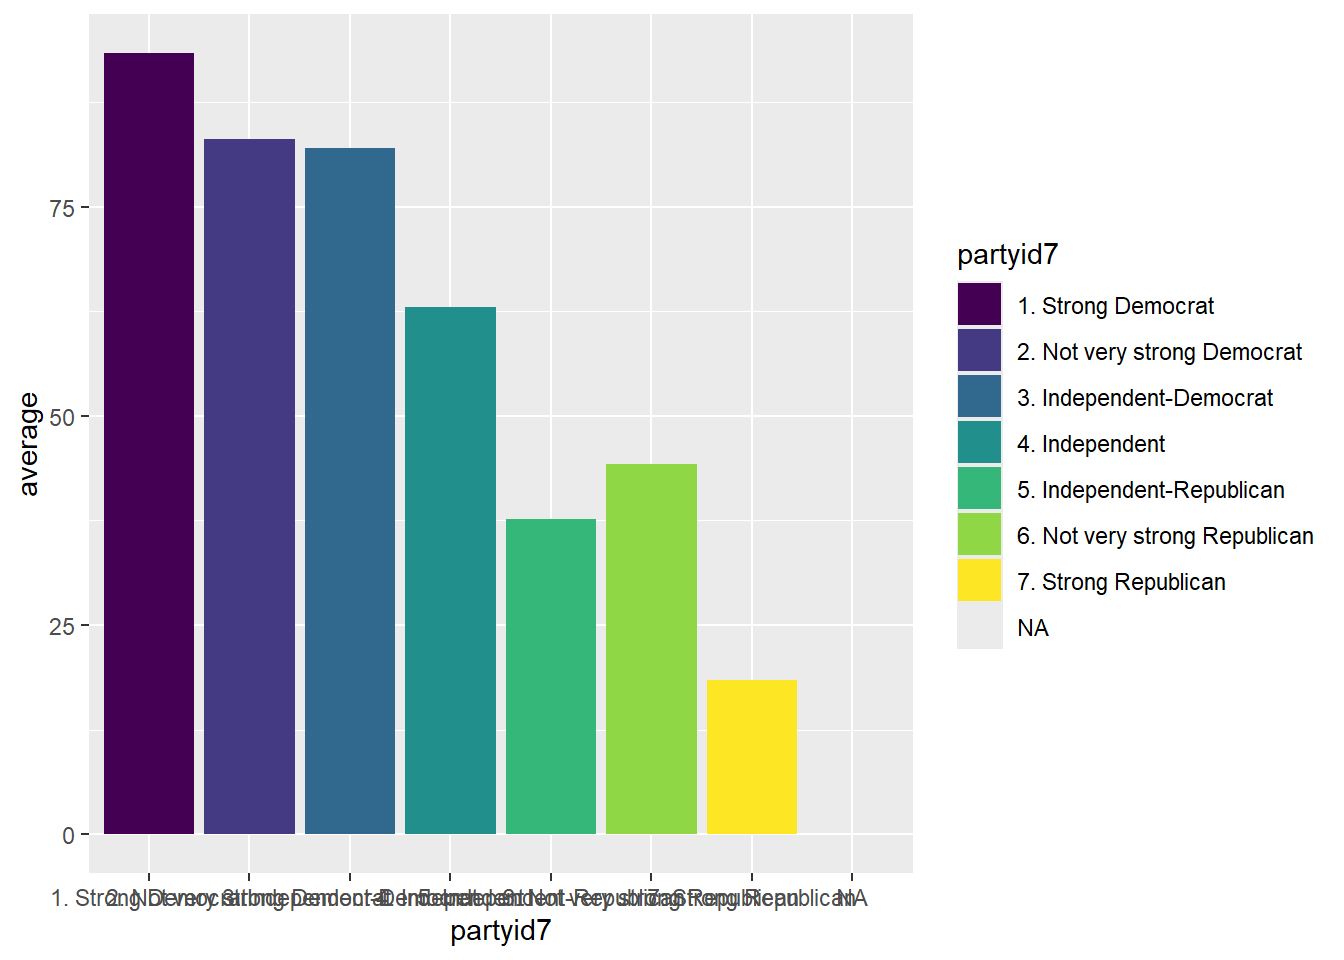
\includegraphics{psc-253-manual_files/figure-latex/unnamed-chunk-97-1.pdf}

\hypertarget{troubleshooting-38}{%
\subsection{Troubleshooting}\label{troubleshooting-38}}

\begin{itemize}
\tightlist
\item
  Make sure that you use the summary dataset instead of the larger dataset.
\item
  If there are errors in making the summary dataset, then there will be problems in the plot.
\item
  Remember that the name of the dependent variable in the plot is the name that you created in the \texttt{summarise()} when creating the summary data.
\item
  You need to load the \texttt{tidyverse} package.
\end{itemize}

  \bibliography{book.bib,packages.bib}

\end{document}
